\documentclass [11pt,twoside]{article}
\usepackage[utf8]{inputenc}
\usepackage[T1]{fontenc}

%Page margins, header and footer positions
\usepackage{geometry}
 \geometry{
 a4paper,
 total={210mm,297mm},
 left=25mm,
 right=25mm,
 top=30mm,
 bottom=25mm,
 headsep=7mm}

\interfootnotelinepenalty=10000

%To display filling dots in the TOC for all entries
\usepackage[titles]{tocloft}
\renewcommand{\cftsecleader}{\cftdotfill{\cftdotsep}}

%Define new header and footer style
\usepackage{fancyhdr}

\pagestyle{fancy}
\fancyhf{}
\lhead{\color{Gray}{\small{Travlendar+ project by YOUR NAMES}}}
\lfoot{\textcolor{Gray}{\small{Copyright © 2017, YOUR NAMES – All rights reserved}}}
\rfoot{\textcolor{Gray}{\thepage}}
\renewcommand{\headrulewidth}{0pt}

%PACKAGES
\usepackage{wasysym}
\usepackage{pifont}

\newcommand{\supported}{\ding{52}\xspace}
\newcommand{\unsupported}{\ding{55}\xspace}
\newcommand{\partsupported}{\textcolor{black!40}{\ding{52}}\xspace}
\newcommand{\lowsupported}{\textcolor{black!20}{\ding{52}}\xspace}
\newcommand{\unknowsupported}{\textbf{?}\xspace}

%Font: Times
\usepackage{times}
%Change monospaced font
\renewcommand{\ttdefault}{lmtt}

%tables
\usepackage{tabu}
\usepackage{tabularx}
\usepackage{ltablex}
\usepackage{longtable}
\usepackage{float} % To allow the use of H modifier in long tables

%landscape mode
\usepackage{pdflscape}
\usepackage{rotating}
\usepackage{caption}

%make landscape mode be sensitive to even and odd pages
%start
\def\myrotate{\ifodd\c@page\else-\fi 90}
\makeatletter
\global\let\orig@begin@landscape=\landscape%
\global\let\orig@end@landscape=\endlandscape%
\gdef\@true{1}
\gdef\@false{0}
\gdef\landscape{%
    \global\let\within@landscape=\@true%
    \orig@begin@landscape%
}%
\gdef\endlandscape{%
    \orig@end@landscape%
    \global\let\within@landscape=\@false%
}%
\@ifpackageloaded{pdflscape}{%
    \gdef\pdf@landscape@rotate{\PLS@Rotate}%
}{
    \gdef\pdf@landscape@rotate#1{}%
}
\let\latex@outputpage\@outputpage
\def\@outputpage{
    \ifx\within@landscape\@true%
        \if@twoside%
            \ifodd\c@page%
                \gdef\LS@rot{\setbox\@outputbox\vbox{%
                    \pdf@landscape@rotate{-90}%
                    \hbox{\rotatebox{90}{\hbox{\rotatebox{180}{\box\@outputbox}}}}}%
                }%
            \else%
                \gdef\LS@rot{\setbox\@outputbox\vbox{%
                    \pdf@landscape@rotate{+90}%
                    \hbox{\rotatebox{90}{\hbox{\rotatebox{0}{\box\@outputbox}}}}}%
                }%
            \fi%
        \else%
            \gdef\LS@rot{\setbox\@outputbox\vbox{%
                \pdf@landscape@rotate{+90}%
                \hbox{\rotatebox{90}{\hbox{\rotatebox{0}{\box\@outputbox}}}}}%
            }%
        \fi%
    \fi%
    \latex@outputpage%
}
\makeatother
%end

%graphics
\usepackage{graphicx}
\usepackage[dvipsnames, table]{xcolor}
%If you upload images from PC, you need to insert code for the path here (different for Windows and Unix OS)

%References
%\usepackage{xpatch}
%\usepackage[backend=biber, style=numeric, citestyle=numeric, sorting=none]{biblatex}
%\addbibresource{main.bib}

%Other
\usepackage{ifthen}
\usepackage{xspace}
\usepackage{enumitem}
\usepackage{amssymb}
\usepackage[hidelinks]{hyperref}
\newcommand{\comment}[1]{{\color{Red}$\blacktriangleright$ Comment: #1 $\blacktriangleleft$}}


% Some utilities\ldots
\usepackage{soul}
\usepackage{tikz}

\usetikzlibrary{calc}
\usetikzlibrary{decorations.pathmorphing}


\makeatletter

\newcommand{\defhighlighter}[3][]{%
  \tikzset{every highlighter/.style={color=#2, fill opacity=#3, #1}}%
}

\defhighlighter{yellow}{.5}

\newcommand{\highlight@DoHighlight}{
  \fill [ decoration = {random steps, amplitude=1pt, segment length=15pt}
        , outer sep = -15pt, inner sep = 0pt, decorate
       , every highlighter, this highlighter ]
        ($(begin highlight)+(0,8pt)$) rectangle ($(end highlight)+(0,-3pt)$) ;
}

\newcommand{\highlight@BeginHighlight}{
  \coordinate (begin highlight) at (0,0) ;
}

\newcommand{\highlight@EndHighlight}{
  \coordinate (end highlight) at (0,0) ;
}

\newdimen\highlight@previous
\newdimen\highlight@current

\DeclareRobustCommand*\highlight[1][]{%
  \tikzset{this highlighter/.style={#1}}%
  \SOUL@setup
  %
  \def\SOUL@preamble{%
    \begin{tikzpicture}[overlay, remember picture]
      \highlight@BeginHighlight
      \highlight@EndHighlight
    \end{tikzpicture}%
  }%
  %
  \def\SOUL@postamble{%
    \begin{tikzpicture}[overlay, remember picture]
      \highlight@EndHighlight
      \highlight@DoHighlight
    \end{tikzpicture}%
  }%
  %
  \def\SOUL@everyhyphen{%
    \discretionary{%
      \SOUL@setkern\SOUL@hyphkern
      \SOUL@sethyphenchar
      \tikz[overlay, remember picture] \highlight@EndHighlight ;%
    }{%
    }{%
      \SOUL@setkern\SOUL@charkern
    }%
  }%
  %
  \def\SOUL@everyexhyphen##1{%
    \SOUL@setkern\SOUL@hyphkern
    \hbox{##1}%
    \discretionary{%
      \tikz[overlay, remember picture] \highlight@EndHighlight ;%
    }{%
    }{%
      \SOUL@setkern\SOUL@charkern
    }%
  }%
  %
  \def\SOUL@everysyllable{%
    \begin{tikzpicture}[overlay, remember picture]
      \path let \p0 = (begin highlight), \p1 = (0,0) in \pgfextra
        \global\highlight@previous=\y0
        \global\highlight@current =\y1
      \endpgfextra (0,0) ;
      \ifdim\highlight@current < \highlight@previous
        \highlight@DoHighlight
        \highlight@BeginHighlight
      \fi
    \end{tikzpicture}%
    \the\SOUL@syllable
    \tikz[overlay, remember picture] \highlight@EndHighlight ;%
  }%
  \SOUL@
}

\makeatother

% Common abbrev. are set as commands to ensure proper spacing after the dot
\RequirePackage{xspace}
\newcommand{\ie}{i.e.\@\xspace}
\newcommand{\aka}{a.k.a.\@\xspace}
\newcommand{\Ie}{I.e.\@\xspace}
\newcommand{\cf}{cf.\@\xspace}
\newcommand{\Cf}{Cf.\@\xspace}
\newcommand{\eg}{e.g.\@\xspace}
\newcommand{\Eg}{E.g.\@\xspace}
\newcommand{\etal}{et al.\@\xspace}
\newcommand{\etc}{etc.\@\xspace}
\newcommand{\wrt}{w.r.t.\@\xspace}
\newcommand{\Wrt}{W.r.t.\@\xspace}



\date{}


\begin{document}

%TITLE PAGE

\begin{titlepage}


%LOGO

{\begin{table}[t!]
\centering
\begin{tabu} to \textwidth { X[1.3,r,p] X[1.7,l,p] }
\textcolor{Blue}
{\textbf{\small{Travlendar+ project YOUR NAMES}}} & 
\includegraphics[scale=0.5]{Images/PolimiLogo}
\end{tabu}
\end{table}}~\\ [7cm]

%TITLE 

\begin{flushleft}

%Replace the text string with your title
{\textcolor{Blue}{\textbf{\Huge{Requirement Analysis and Specification
        Document}}}} \\ [1cm]

\end{flushleft}

\end{titlepage}

%Define deliverable specific info
%Replace cell contents where needed
\begin{table}[h!]
\begin{tabu} to \textwidth { X[0.3,r,p] X[0.7,l,p] }
\hline

\textbf{Deliverable:} & RASD\\
\textbf{Title:} & Requirement Analysis and Verification Document \\
\textbf{Authors:} & YOUR NAMES \\
\textbf{Version:} & 1.0 \\ 
\textbf{Date:} & 31-January-2016 \\
\textbf{Download page:} & LINK TO YOUR REPOSITORY \\
\textbf{Copyright:} & Copyright © 2017, YOUR NAMES – All rights reserved \\
\hline
\end{tabu}
\end{table}




\setcounter{page}{2}


%------------------------------------------------------------------------------------------------------------------------------------------------
\newpage
\addcontentsline{toc}{section}{Table of Contents}
\tableofcontents
\newpage
\addcontentsline{toc}{section}{List of Figures}
\listoffigures
\addcontentsline{toc}{section}{List of Tables}
\listoftables

%------------------------------------------------------------------------------------------------------------------------------------------------
\clearpage
{\color{Blue}{\section{Introduction}}}
\label{sect:introduction}
\subsection{Purpose}
The purpose of the DD is to provide a strategic guide to develop the project in the correct way, avoiding the errors and the waste of time that could be generated without studiyng the problem and the possible solutions. The document will be given to the development team.
\subsubsection{Scope}
The web platform will provide a system that manage the reports of the parking violations and elaborates the data to retrieve information about streets and cars:
\begin{itemize}
	\item
	Report violation
	\item 
	Report validation
	\item
	Update statistics
	\item
	Manage streets data
	\item
	Different usage between end user and authority
\end{itemize}
\subsection{Definitions, Acronyms, Abbreviations}
\subsubsection{Definitions}
\begin{itemize}
	\item 
	End-user: The end-user is the common user of the application, that take the picture of the violations and send it with all the report data to the Application server.
	\item 
	Authority: The authority are the municipality that will provide the traffic tickets to who commit a violation and can access different data than the end-user.
	\item 
	Web Server: A Web server uses HTTP (Hypertext Transfer Protocol) to provide the files that compose the Web pages to users, in response to their requests, which are forwarded by their hosts' HTTP clients. Dedicated computers and appliances may be referred to as Web servers as well.
	\item 
	Application Server: An application server is a type of server designed to install, operate and host applications and associated services for end users, IT services and organizations.
\end{itemize}
\subsubsection{Acronyms}
\begin{itemize}
	\item
	API: Application Programming Interface
	\item
	DD: Design Document
	\item
	JDBC: Java DataBase Connectivity
	\item
	RASD: Requirements Analysis and Specifications Document
	\item
	RMI: Remote Method Invocation
	\item
	UX: User Experience
	\item
	ANPR: Automatic number-plate recognition, is the portion of the system
	that is able to recognize the license plate number from the pictures prodived
	by users.
	\item
	CUU: Code Unique Unitary
	
\end{itemize}

\subsubsection{Abbreviations}

%------------------------------------------------------------------------------------------------------------------------------------------------
\clearpage
{\color{Blue}{\section{Overall Description}}}
\label{sect:overview}
\subsection{Product perspective}

\subsubsection{Further details on shared phenomena}

\paragraph{Report:}
is composed by the picture regarding violation and by its metadata: type, road or GPS coordinates, date-time and so forth.
The report transfer is done via HTTPS, in order to be encrypted since it contains private data.
Once it is received, the algorithm checks the picture trustfulness.

\paragraph{Authority notification:} it has to contain the data of the violation that authorities can use to generate traffic tickets.

\paragraph{Data and statistics visualization:} crossed data about violations and accidents are used to create the map with colored road according to the number of violations.


\begin{center}
	\begin{tabular}{ | l | p{6cm} | } 
		\hline
		PHENOMENA & SHARED  \\ 
		\hline
		User check his profile &   Yes \\
		\hline
		User sends the photo of a violation & Yes \\ 
		\hline
		SafeStreets retrieve licence plate & No \\ 
		\hline
		SafeStreets retrieve position & Yes \\ 
		\hline
		SafeStreets check reliability of the photo & No \\ 
		\hline
		SafeStreets locate the most unsafe area &  No\\ 
		\hline
		SafeStreets provide suggestions & Yes \\
		\hline
	\end{tabular}
\end{center}

\subsubsection{Domain model}

The platform has to manage different entities. Some of them are linked and they shared data and function.
The entities are: 
\begin{itemize}
\item Users
\item Local authorities
\item Reports about possible violations (now defined as Report)
\item Real violations
\item Statistics
\end{itemize}


When the user see a parking violation, he could take a picture of the involved car (is important that the license plate is visible) and sends it to the system with all the relative information about the type of violation and the road.

All of these information are used to create report entities that are analyzed by the platform’s algorithm.

If the report is genuine, these data can be used by authorities to generate traffic tickets, with their systems.

Furthermore, they can analyze which are unsafe areas or the vehicles that commit the most violation.

Results are also available inside SafeStreets.
The same operation is done automatically by the platform, crossing reports from users and accidents information provided by authorities.


\subsubsection{Class diagram}
\begin{figure}[H]
	\centering
	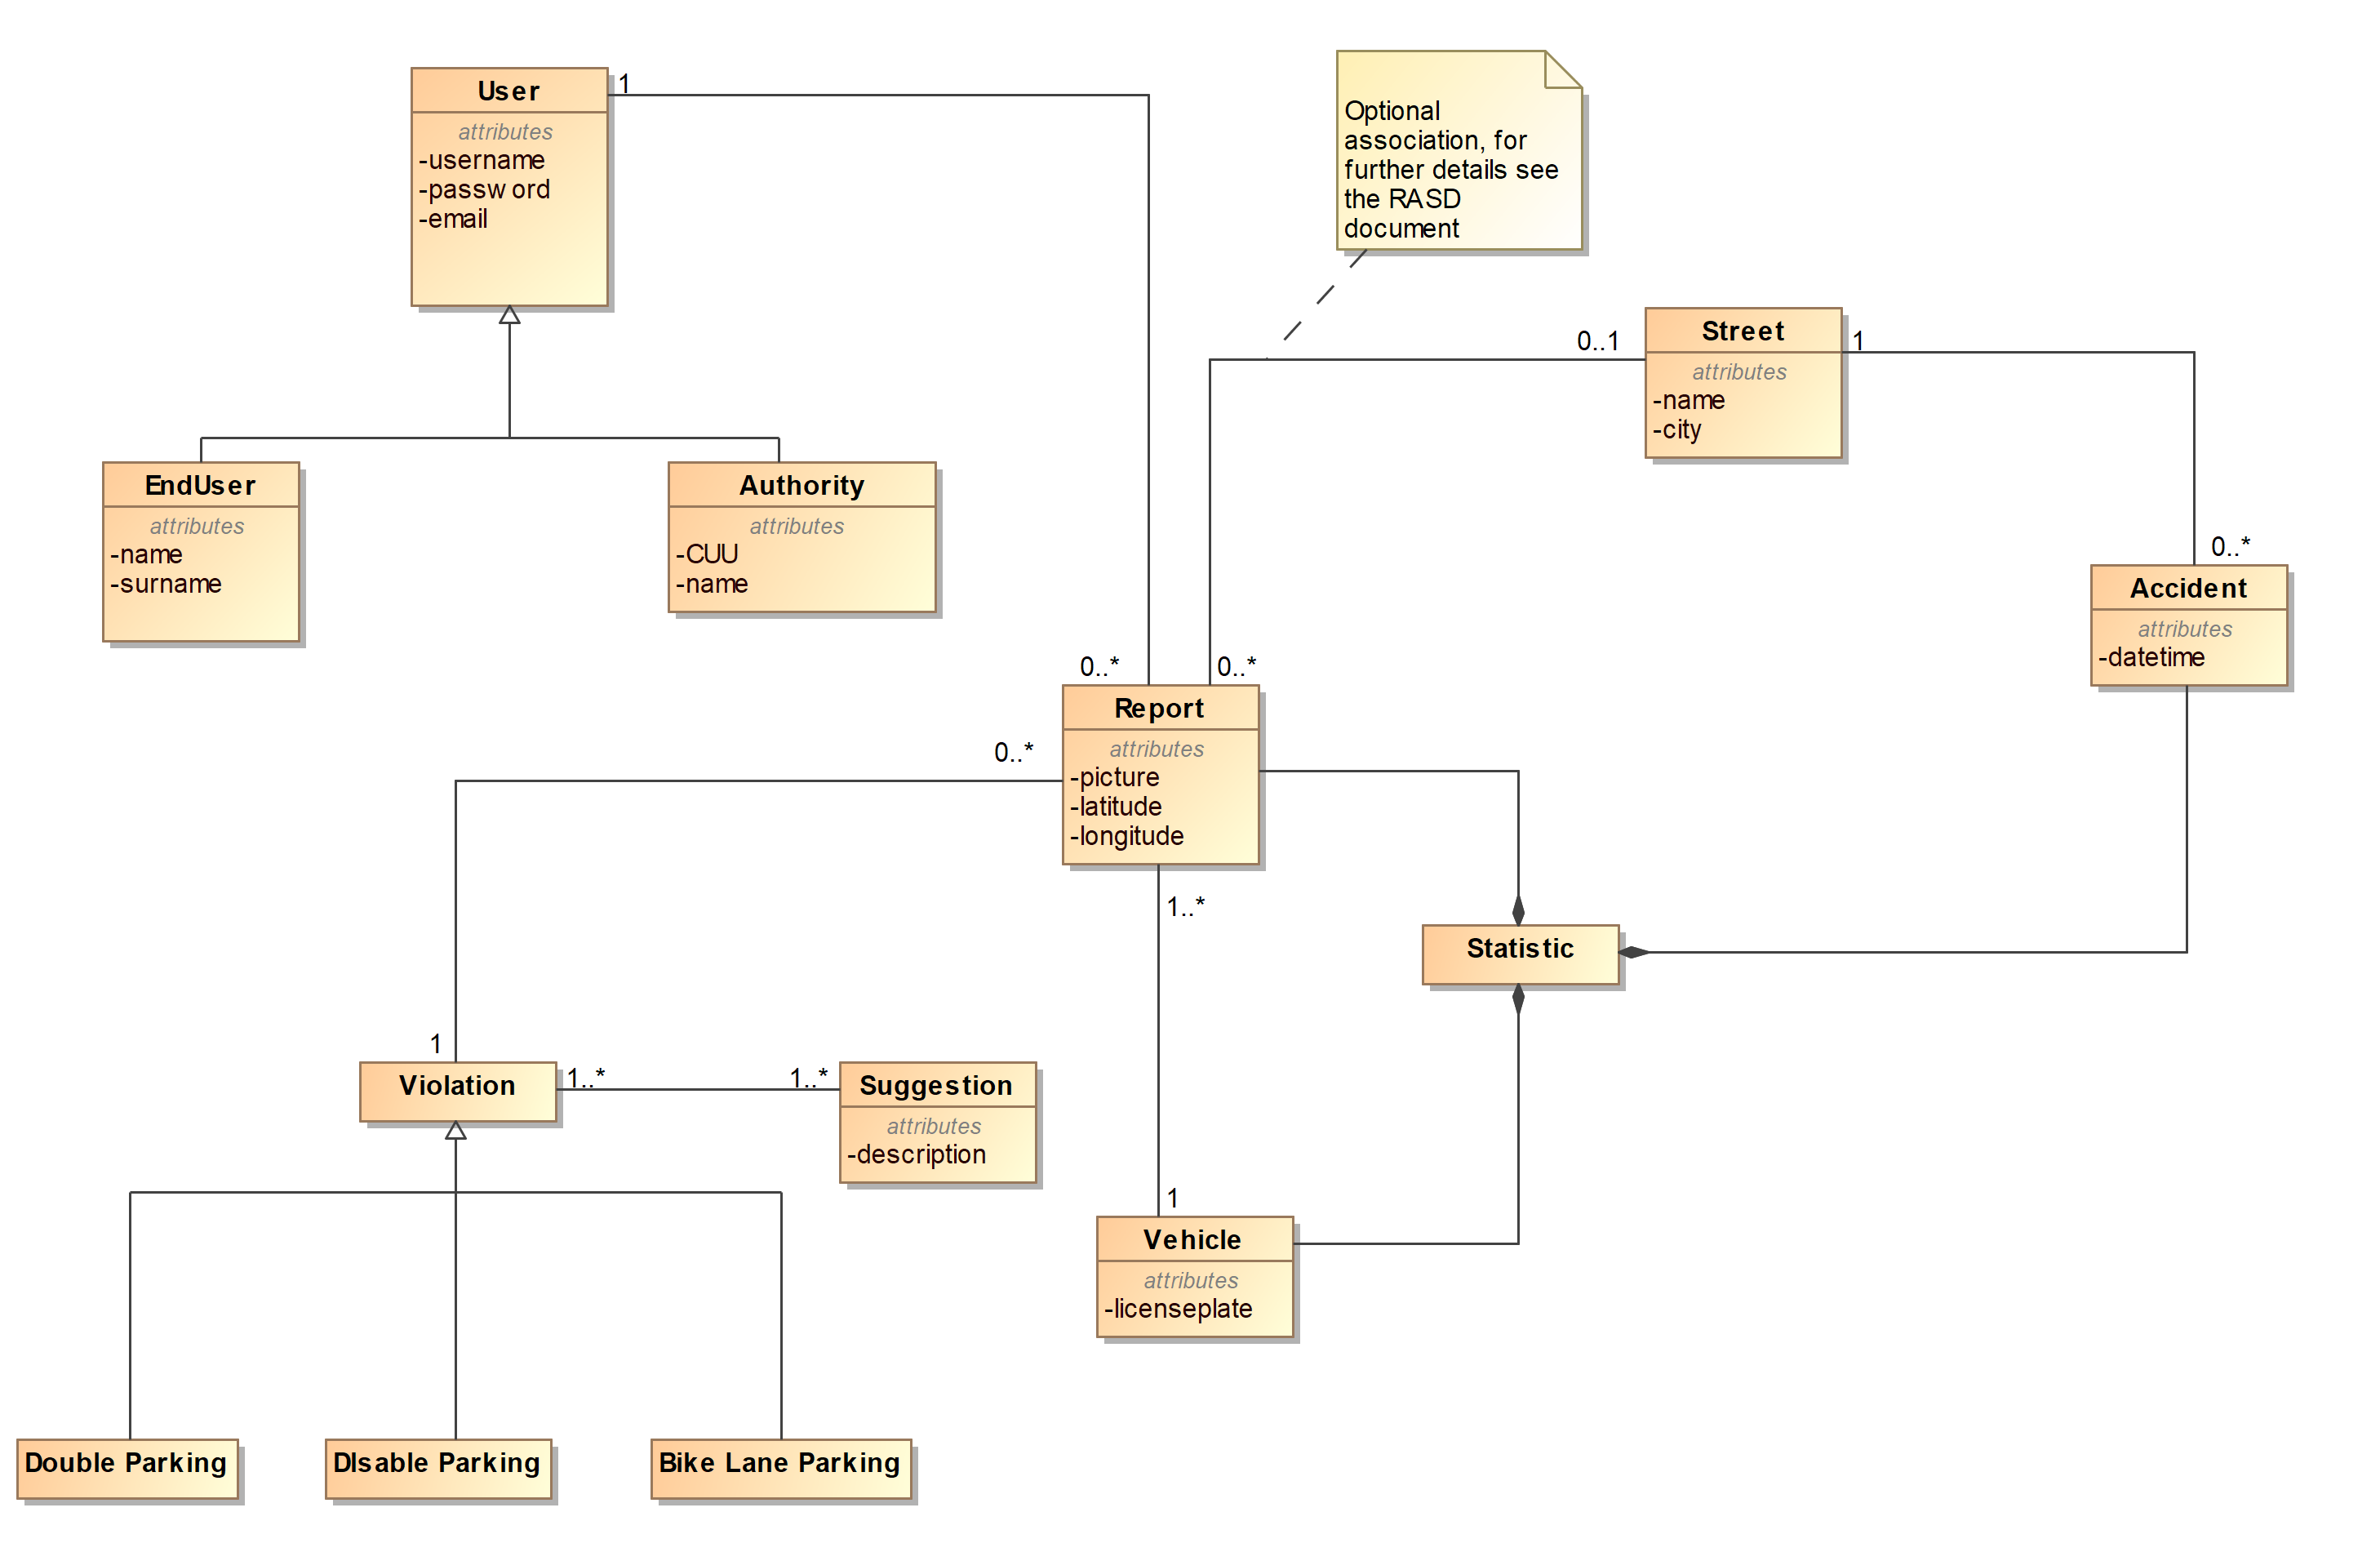
\includegraphics[width=1.12\linewidth]{Images/ClassDiagram.png}
	\caption{Class Diagram}
\end{figure}
The association between Report and Street is optional because we retrieve the position of the report automatically using GPS. Only in case of problem with this operation, we require the address to the user. In this case, SafeStreets calulates the coordinates using the address provided by the user. We use the andress also in case of report made in a place different from the one where the violation occurred. 
\subsubsection{Statechart}
\begin{figure}[H]
	\centering
	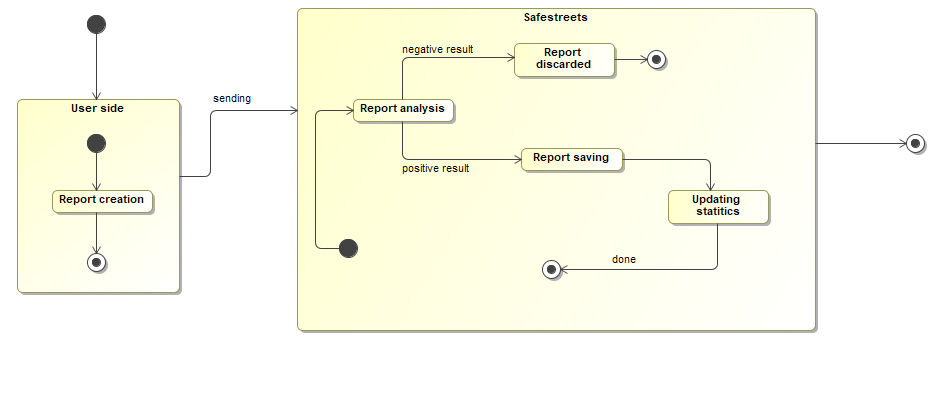
\includegraphics[width=1.12\linewidth]{Images/ReportLifeCycle.png}
	\caption{Report life cycle}
\end{figure}
\begin{figure}[H]
	\centering
	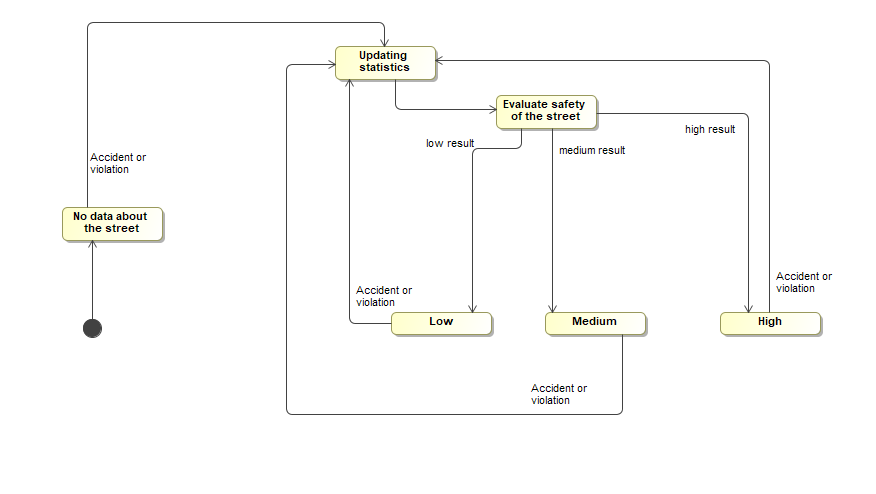
\includegraphics[width=1.12\linewidth]{Images/StreetLifeCycle.png}
	\caption{Street life cycle}
\end{figure}
\newpage

\subsection{Product functions}
Considering the objectives requested by SafeStreets, main functions are described below:

\subsubsection{Notify Traffic Violations RE.1}
The main requirement of the application is to provide users a smart and effortless tool to notify authorities when traffic violations occur.

Users are able to select the type of violation, providing the name of the street, or using their GPS position, and uploading a picture containing the license plate that will be read by an algorithm.

Furthermore, in order to increase the reliability of the system we require the manual insertion of the license plate. When the license will be retried from the image, the result will be compared with the number sended by the user. If the comparison will not return equality, the report will be discarded.

\subsubsection{License Plate Recognition RE.2}
License plate recognition functionality is crucial for SafeStreets, from the license plate we can get information about the owner, the vehicle and its specs.

The fact that there isn't a human being responsible for manually recognizing license plates is important for the scalability, when the application will be used on a large scale.

Automatic number-plate recognition (ANPR) technology consists in seven primary algorithms that the software requires: Plate localization, Plate orientation and sizing, Normalization, Character segmentation, Optical character recognition, Geometrical analysis, Averaging of the recognized values to produce a more reliable or confident result.

Due to the fact that the image will be widely analyzed, it must be in high resolution with no blur and in a good lighting context.

\subsubsection{Data Collection RE.3}
Due to the fact that data is the most valuable asset of modern industry, data collection is important for all statistics, information and data visualization that SafeStreets provides.

It collects data coming from different sources: users inputs, municipality and police databases.
Data collection involve several practices about correctness and security.

\subsubsection{Data Visualization RE.4}
A portion of the application is dedicated to data visualization by showing a map on which the streets/areas are colored according to the frequency of violations and accidents, compared to the average numbers: 
\begin{itemize}
\item red = high
\item yellow = medium
\item green = low
\item white = no data
\end{itemize}

Also there is a part of the UI where authorities can see statistics about vehicles and their violations.

\subsubsection{Data Sets Analysis RE.5}
The functionality of data analysis is crucial for finding patterns in data sets.

\subsubsection{Suggest Possible Interventions RE.6}
Thanks to data sets analysis, SafeStreets can suggest possible interventions for already identified "high-violation" streets.

For each type of violation is assigned one or more possible interventions that will help to decrease the occurrence of that specific violation.


\subsubsection{Information Integrity RE.7}
Data integrity is defined as maintenance and assurance of data consistency over its entire life-cycle.

Ensuring that data are correct and information are never altered is crucial, because local police could take the information about violations coming from SafeStreets.

\subsubsection{Generating Traffic Tickets RE.8}
This functionality is not an internal feature of the application. 

Our scope is to provide the police, data about violations and with this information the municipality could generate traffic tickets with their own systems..

For this reason SafeStreets exposes REST API endpoints to allow authenticated authority users, in this case the police, to get violations information.


\subsection{User characteristics}

The following actors are the users of this application:

\begin{itemize}
	\item End users
\end{itemize}

The end user is a person who, after the sign up, can use SafeStreets to notify traffic violations, consult statistics and see the map with violation information for each street.

\begin{itemize}
	\item Authorities:
	\subitem Municipality
	\subitem Local police
\end{itemize}


Authority is an organization who, after a different sign up from end users, using CUU code, can use SafeStreets to get information about traffic violations for generating traffic tickets, consult possible interventions suggested, see statistics and the map with violation information for each street.
Also they can provide their data to SafeStreets, in this way our platform is able to cross authorities data with its own data.

\subsubsection{Assumptions, dependencies and constraints}
	In this document it is supposed that:
\begin{itemize}
	\item 
	in the country where SafeStreets will be used, the law admits these type of systems.
	
	\item 
	we consider only the following type of violations
	\subitem
	Double parking
	\subitem
	Disable parking
	\subitem
	Bike lane parking
\end{itemize}





%------------------------------------------------------------------------------------------------------------------------------------------------
\clearpage
{\color{Blue}{\section{Specific Requirements}}}
\label{sect:requirements}

\subsection{External Interface Requirements}
\subsubsection{User interfaces}
The following mocks describe the application UI create after the process (UX) of defining how users interact with SafeStreet:

	\begin{figure}[H]
		\centering
		\begin{minipage}[b]{0.40\textwidth}
			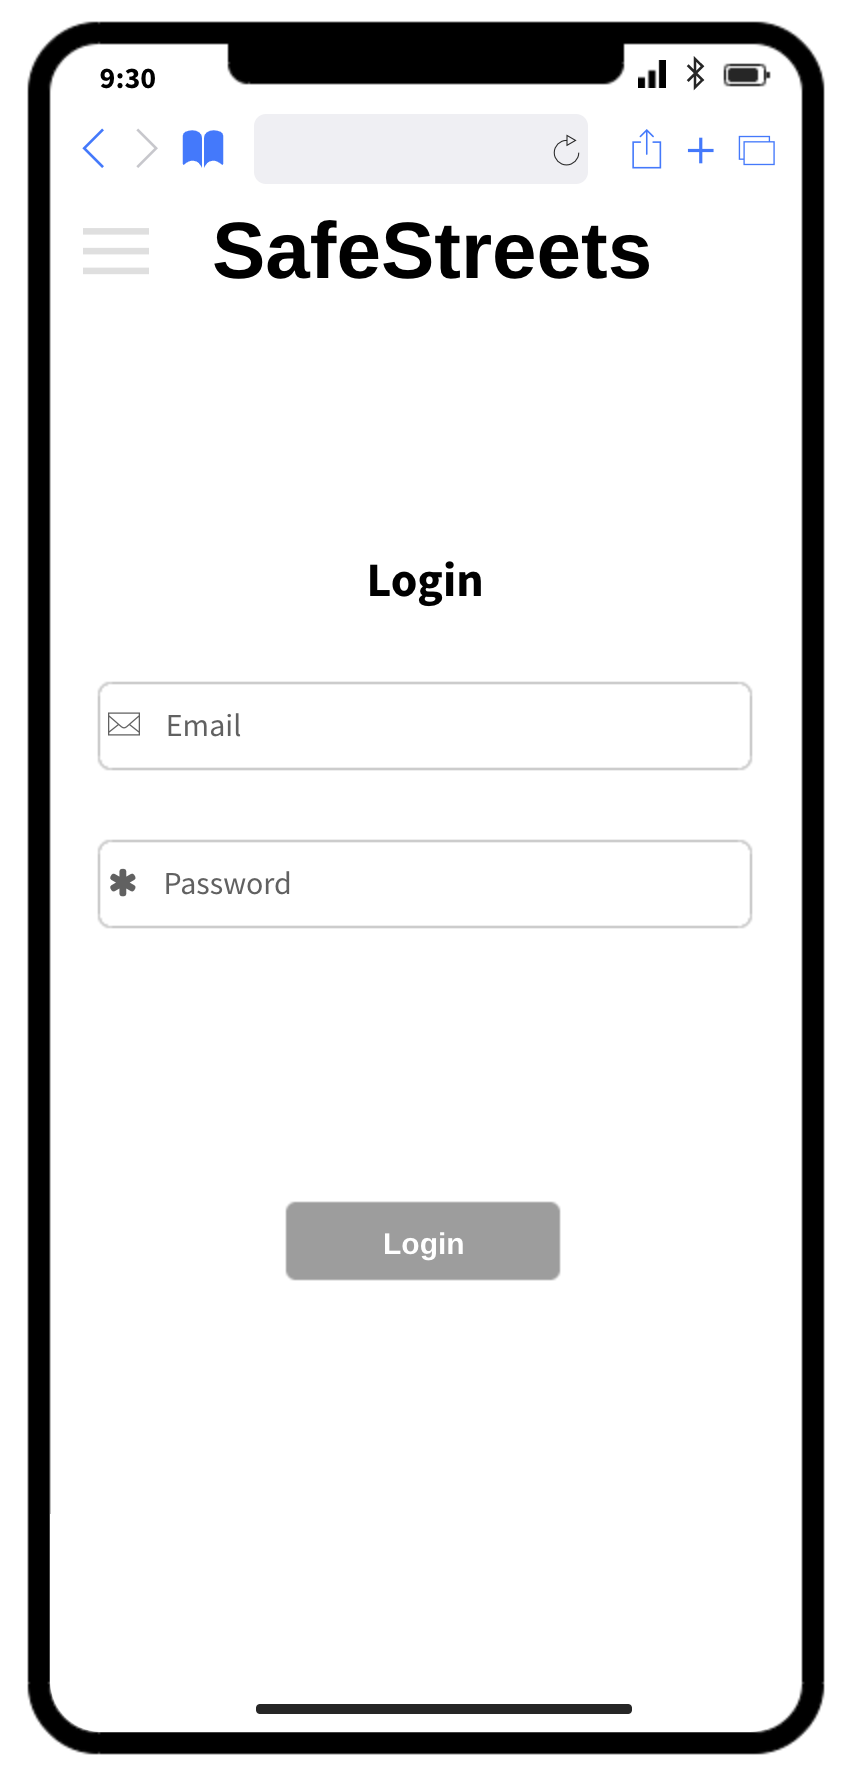
\includegraphics[width=\textwidth]{Images/login.png}
			\caption{Login form}
		\end{minipage}
		\hfill
		\begin{minipage}[b]{0.4\textwidth}
			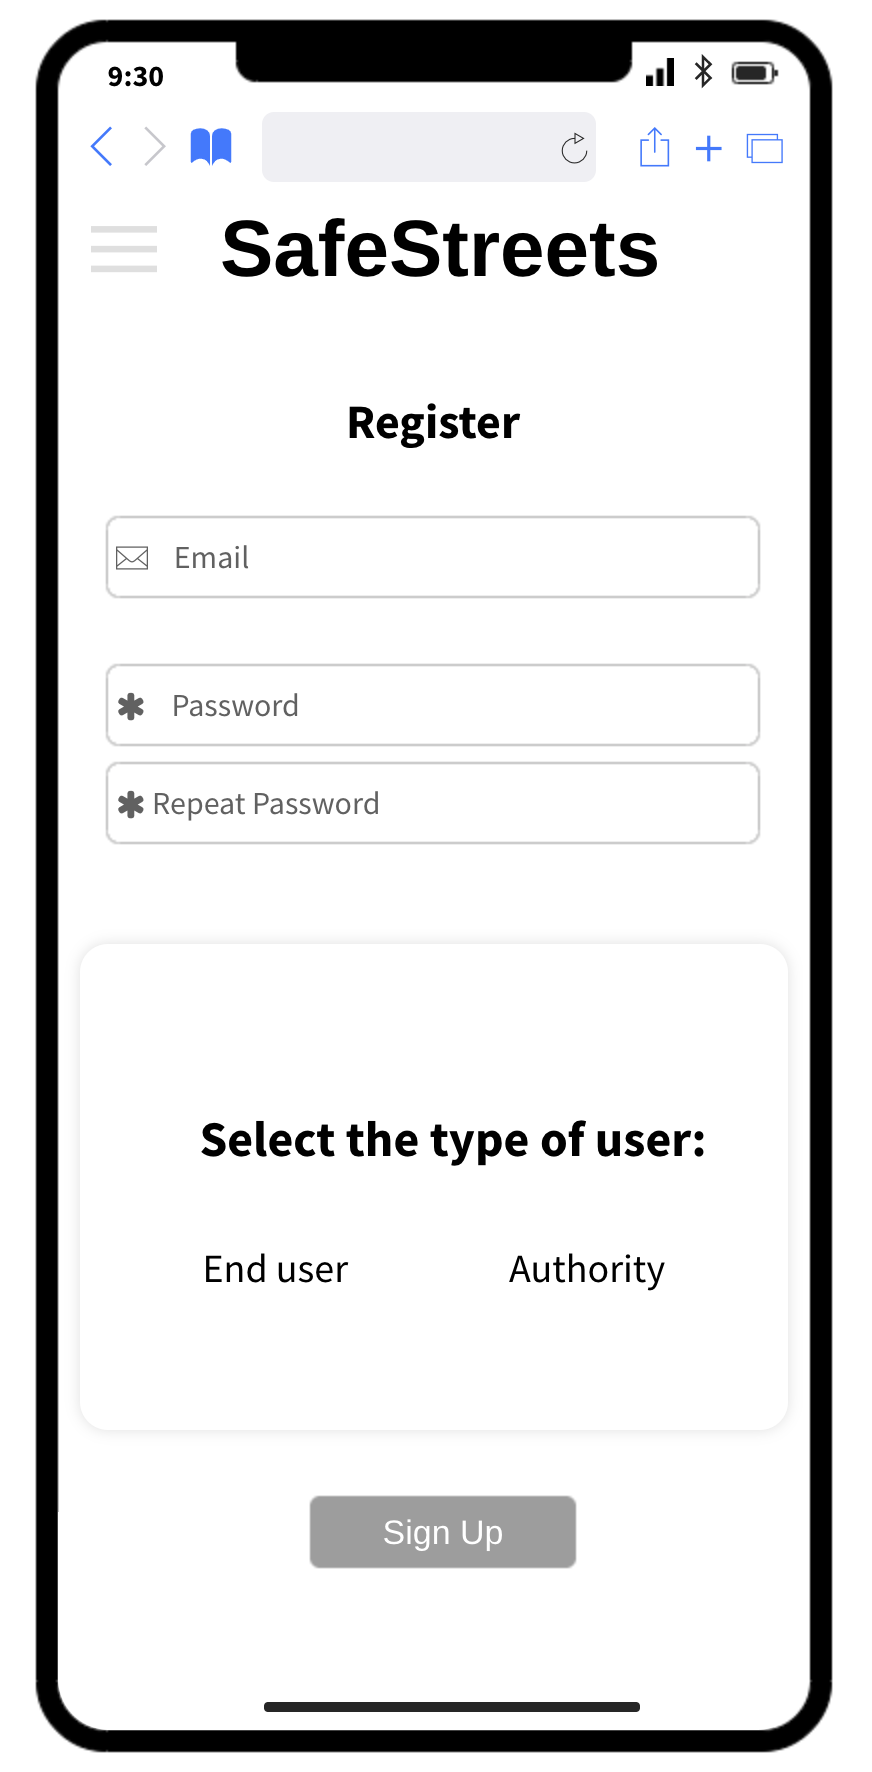
\includegraphics[width=\textwidth]{Images/registration.png}
			\caption{Registration form}
		\end{minipage}
	\end{figure}
	
		\begin{figure}[H]
		\centering
		\begin{minipage}[b]{0.40\textwidth}
			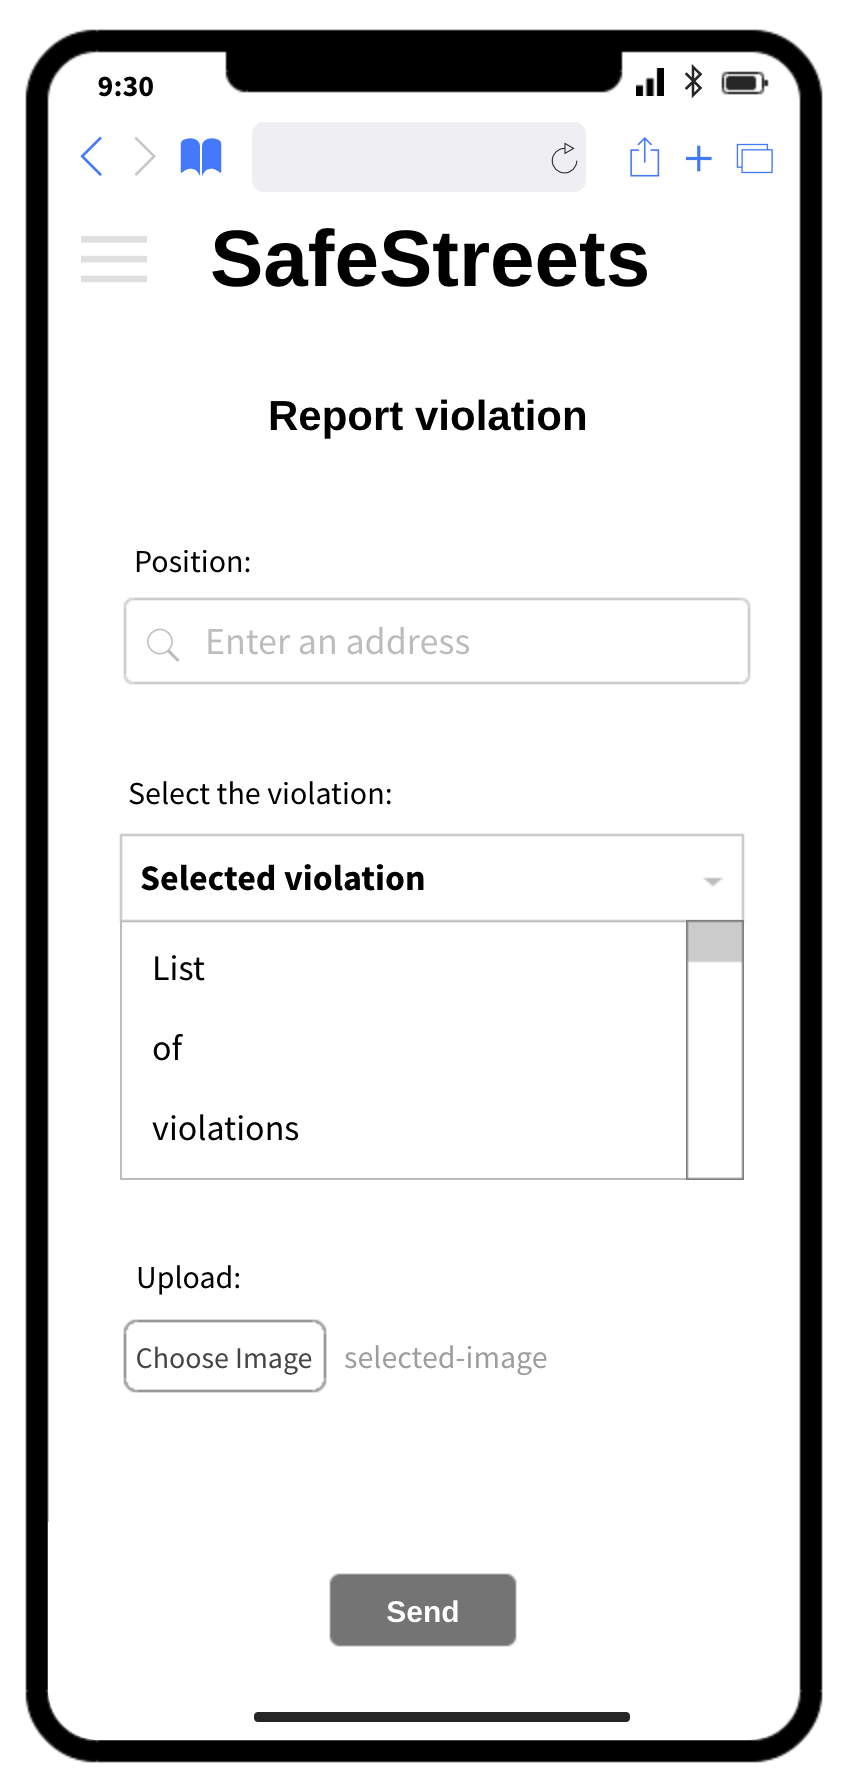
\includegraphics[width=\textwidth]{Images/report.png}
			\caption{User send violation report}
		\end{minipage}
		\hfill
		\begin{minipage}[b]{0.4\textwidth}
			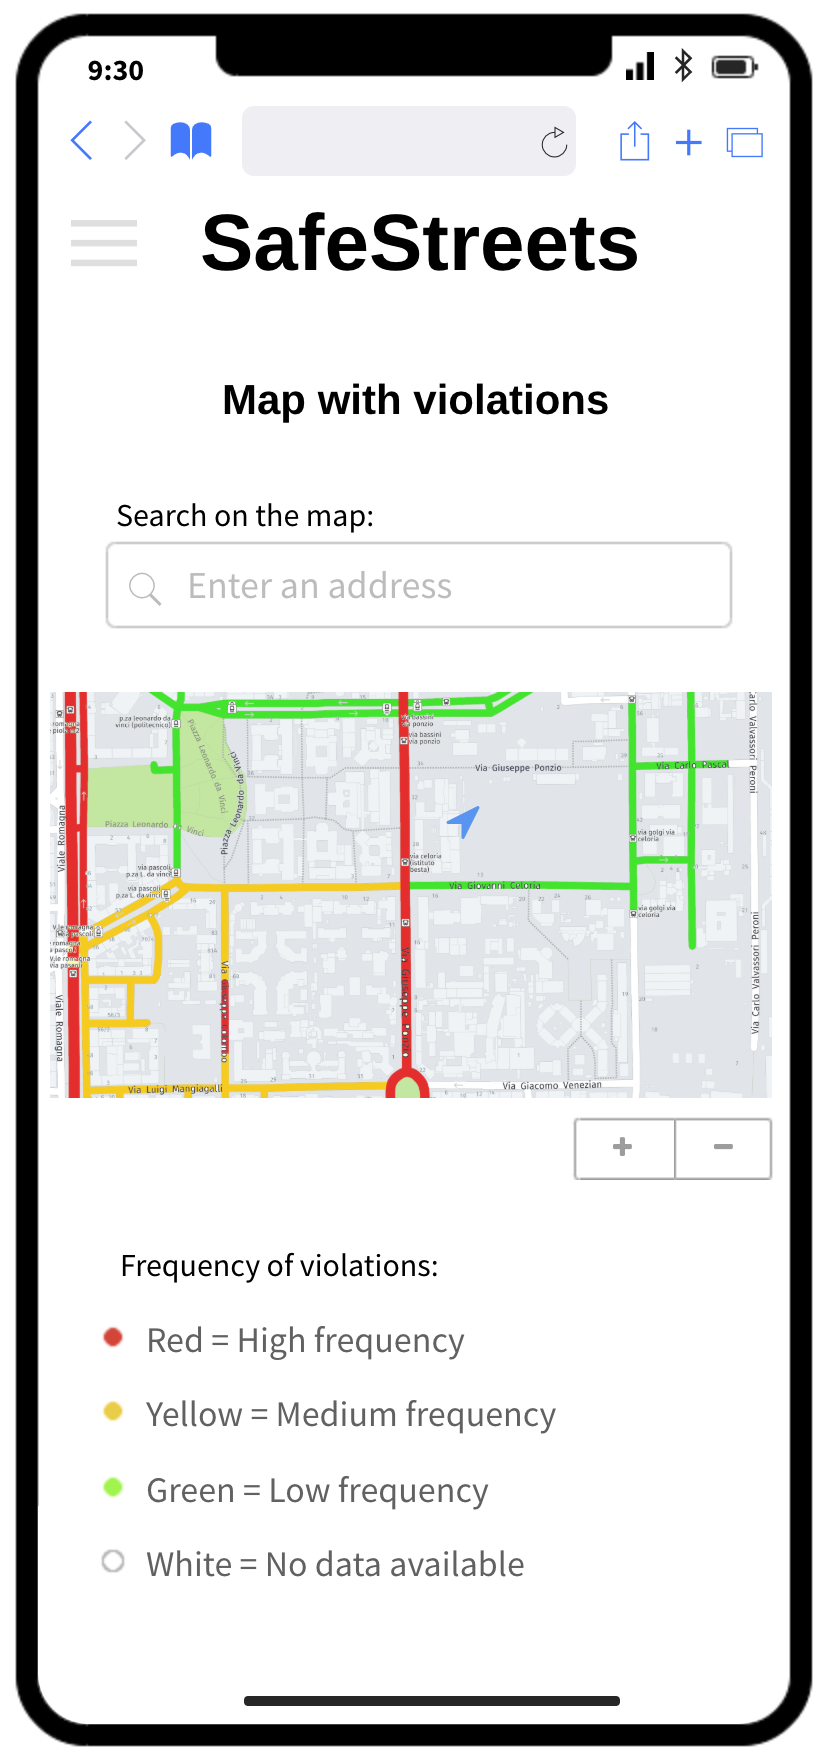
\includegraphics[width=\textwidth]{Images/violationsMap.png}
			\caption{Map showing violations}
		\end{minipage}
	\end{figure}

	\begin{figure}[H]
	\centering
	\begin{minipage}[b]{0.40\textwidth}
		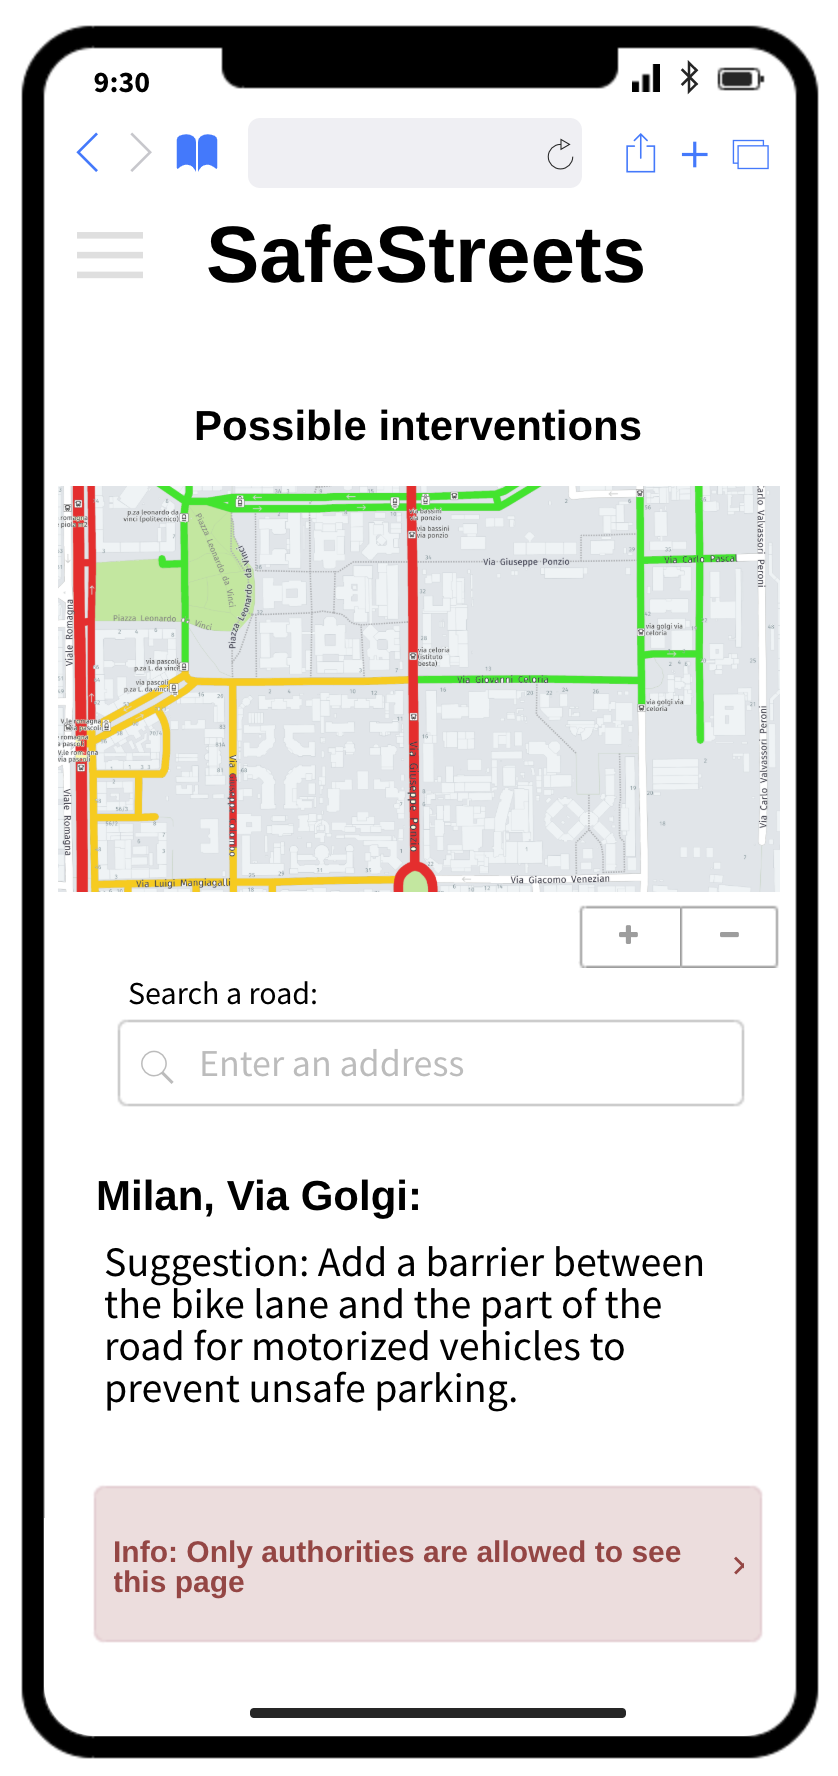
\includegraphics[width=\textwidth]{Images/interventions.png}
		\caption{Suggestion for possible interventions}
	\end{minipage}
	\hfill
	\begin{minipage}[b]{0.4\textwidth}
		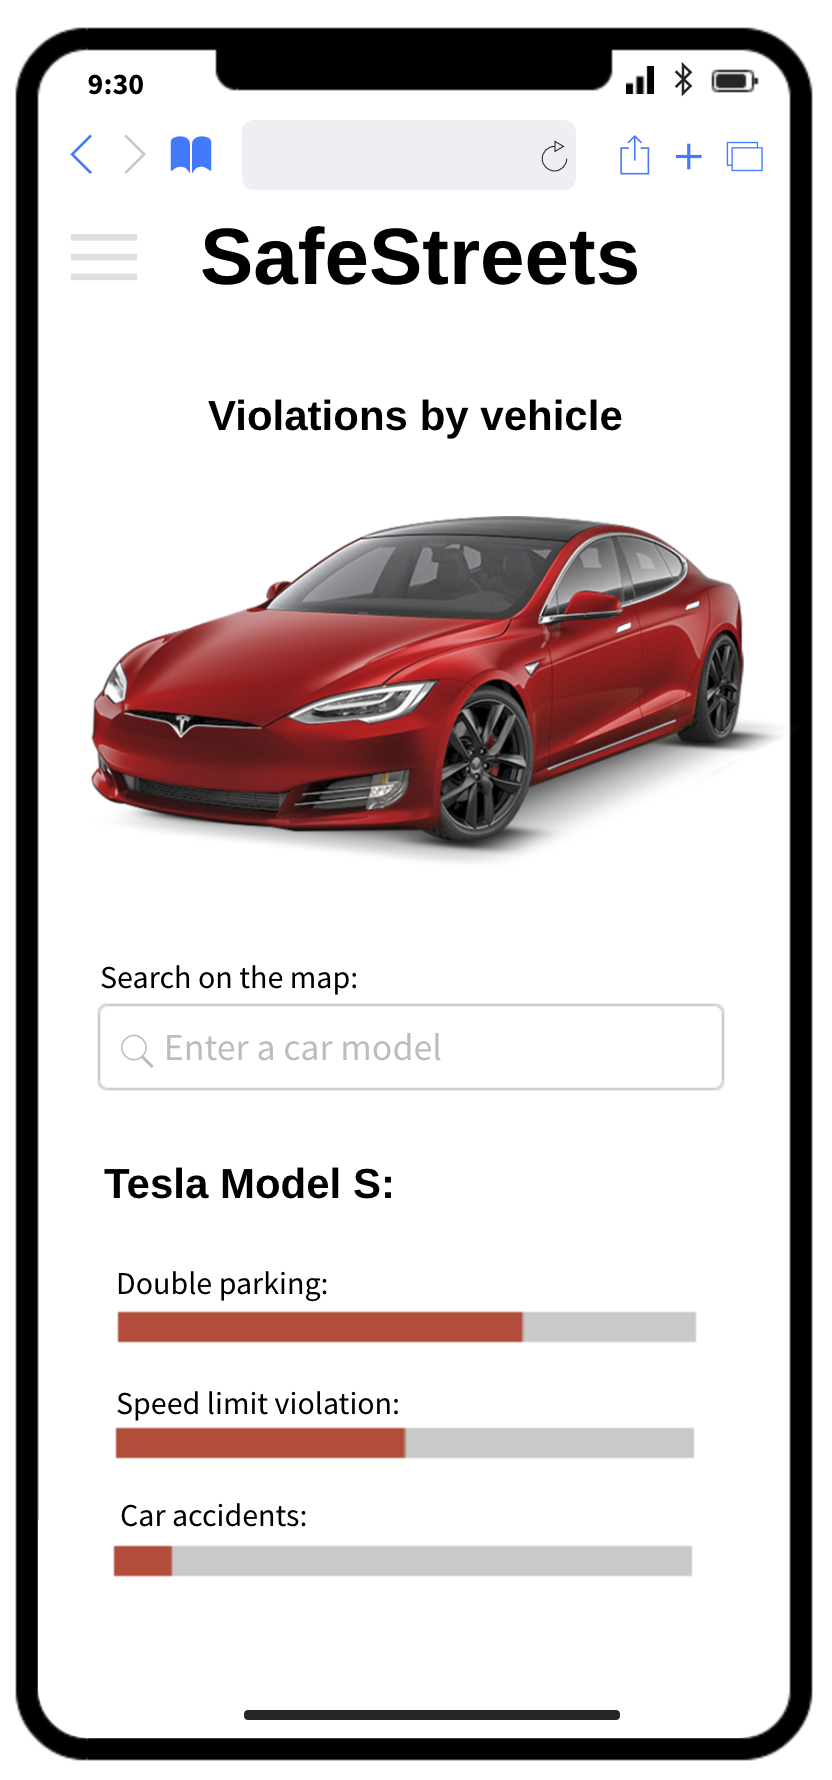
\includegraphics[width=\textwidth]{Images/vehicle.png}
		\caption{Violations by vehicle}
	\end{minipage}
\end{figure}

\subsubsection{Hardware interfaces}

\subsubsection{Software interfaces}
The system functionalities are provided without using third part application except for the CUU (Codice Univoco Ufficio) verification. This functions is made by an external web service provided by IndicePA. The code is required during the authorities registration to ensure their identity.
The external API are exposed only for authorities application and the implentation details will be shown in the design document.

\subsubsection{Communication interfaces}
Any communication functionality takes place via internet with HTTP protocol.
More in details, the protocol used is HTTPS, to allow protection and privacy.
This protocol will be used for both access to the web-application and REST communication.

\subsection{Design constraints}
\subsubsection{Standards compliance}
Part of the information collected by Safestreet (ex: license plate) are sensitive. For this reason the project is subject to the General Data Protection Regulation (GDPR). One of the technique used by the system to protect these important information is the creation of different type of user. For example normal account can only send information while authorities have a different account that is able to access to the data colleceted and generated.

\subsubsection{Hardware limitations}
The application is based on retrieving data from the photos sent by the user. Obviously the camera of the devices is a crucial aspect to consider during the design process. For this reason a minimun resolution of the sensor is required to install the application.The identification of this value will be done during design phase and will be written in the design document.
An other constraint is generated by the precision of the gps sensor of the device. Since the impact is smaller than the image resolution, the requirement is not so strict. 

\subsubsection{Any other constraint}
Safestreet works with violations and traffic tickets so it has to deal with law and regulation implications.
For this aspect see the specific domain assumption. 
Furthermore we have to consider the possible improper use of the platform. To prevent it Safestreet do some specific control on the images and is able to detect editing or repeated photos of the same violations. The implementation of this part will be done with some external algorithm and will be detailed in the design document.

\subsection{Functional requirements}
\subsubsection{Definition of use case diagram}
The use case diagrams provide a vision of the uses that can be done with the platform. They show the relationship between the actors and the use that every actor made with the software to reach the goals.

\subsubsection{Scenario 1}
Paul wants to sign up to SafeStreet platform. He has to insert his personal data (name, surname,place,mail etc.) and optionally also the car license plate. He will recieve a confirm mail and can use the platform.
\subsubsection{Scenario 2}
Bob is coming back to his car when he notice that someone has parked in double row and he can’t move. He log in into the safestreet app and he take a picture of the car to report it to the platform which analize the reporting and, in case it is true,it  could generate a traffic ticket and store the data to generate statistics.

\subsubsection{Scenario 3}
Luke is walking on the sidewalk when he see that a young guy is parking on a park reserved for disable.
Luke take a picture of the car and report it to the safestreet platform which analize the reporting and in case it could generate a traffic ticket and store the data to generate statistics.

\subsubsection{Scenario 4}
Mark has submitted a report to the safestreet platform, and he want to check if it has been accepted or declined.
He logs in into the app, he accesses to his reserved area and next to his report there is the status of message sent.

\subsubsection{Scenario 5}
Bill wants to check if someone has made a report on his car. He logs in into the platform and get the access to his profile where he can check if there is any traffic ticket for his car.

\subsubsection{Scenario 6}
The local authority wants to check which are the streets with more reports. They log in into the platform and access to their personal area where they can check the street status. They can set the color of the street based on the reports they recieve but also the platform automatically change the color of the streets based on the reports that recieve through the app.

 
\subsubsection{Scenario 7}
The local authority wants to check which are the vehicle with more reports. They log in into the platform and access to their personal area where they can check the cars that have the most reports assigned. They can set the color of the cars based on the reports they recieve but also the platform automatically change the color of the cars based on the reports that recieve through the app.

\subsubsection{Scenario 8}
The system recieves the photos from the users and have to check if they are true or fake. It runs an alghoritm that can detect if the photo is real or it has been modified. In the first case, the report will be stored and can be generate a traffic ticket. In the second case the report will be discarded.

\subsubsection{Scenario 9}
The local authority have to relase a traffic ticket in case of a user made an infringement. The platform auto-generate the trafic tickets when a report result real, and the local authority recieve a notify.

\subsection{Description of use case scenarios}
\subsubsection{Description scenario 1}


\begin{center}
	\begin{tabular}{ | l | p{6cm} | } 
		\hline
		ACTORS & Visitors  \\ 
		\hline
		GOALS & Sign up  \\ 
		\hline
		INPUT CONDITION & Personal data (name, surname, mail, telephone number, place where he lives, car license plate etc.)  \\ 
		\hline
		EVENTS FLOW & The user from the home page clicks on sign up. He inserts all of his information and if it is all correct he will recive an email of confirm.  \\ 
		\hline
		OUTPUT CONDITION & The user can now log in and use all the function that the user can do on the platform.  \\ 
		\hline
		EXCEPTIONS & Data incorrect, user already exists, mail already exists. All of this exceptions will be notified instantly to the user. \\ 
		\hline
	\end{tabular}
\end{center}

\subsubsection{Description scenario 2}

\begin{center}
	\begin{tabular}{ | l | p{6cm} | } 
		\hline
		ACTORS & User  \\ 
		\hline
		GOALS & Report a violation  \\ 
		\hline
		INPUT CONDITION & Type of violation (double row park), name of the street,  \\ 
		\hline
		EVENTS FLOW & The user take a picture of the car that has done the violation. The system use an algorithm to read the car license plate and then store all the informations once it is established that the photo isn't fake.  \\ 
		\hline
		OUTPUT CONDITION & The violation has been stored with all the data, it will be generated a traffic ticket, and the local authority can decide to highlight who has made the violation or the street. \\ 
		\hline
		EXCEPTIONS & Data incorrect or fake photo. The report will be discarded and no traffic ticket will be generated.  \\ 
		\hline
	\end{tabular}
\end{center}

\subsubsection{Description scenario 3}

\begin{center}
	\begin{tabular}{ | l | p{6cm} | } 
		\hline
		ACTORS & User  \\ 
		\hline
		GOALS & Report a violation  \\ 
		\hline
		INPUT CONDITION & Type of violation (wrong park), name of the street,  \\ 
		\hline
		EVENTS FLOW & The user take a picture of the car that has done the violation. The system use an algorithm to read the car license plate and then store all the informations once it is established that the photo isn't fake.  \\ 
		\hline
		OUTPUT CONDITION & The violation has been stored with all the data, it will be generated a traffic ticket, and the local authority can decide to highlight who has made the violation or the street. \\ 
		\hline
		EXCEPTIONS & Data incorrect or fake photo. The report will be discarded and no traffic ticket will be generated.  \\ 
		\hline
	\end{tabular}
\end{center}

\subsubsection{Description scenario 4}

\begin{center}
	\begin{tabular}{ | l | p{6cm} | } 
		\hline
		ACTORS & User  \\ 
		\hline
		GOALS & Check report status  \\ 
		\hline
		INPUT CONDITION & User credentials  \\ 
		\hline
		EVENTS FLOW & The user log in into the platform. He accesses to his personal area and he can check the status of his report \\ 
		\hline
		OUTPUT CONDITION & Report status \\ 
		\hline
		EXCEPTIONS & The user hasn't made any report. The system show a messagge that the list of the reports is empty.  \\ 
		\hline
	\end{tabular}
\end{center}

\subsubsection{Description scenario 5}

\begin{center}
	\begin{tabular}{ | l | p{6cm} | } 
		\hline
		ACTORS & User  \\ 
		\hline
		GOALS & Check his profile  \\ 
		\hline
		INPUT CONDITION & User credentials  \\ 
		\hline
		EVENTS FLOW & The user log in into the platform. He accesses to his personal area and he can check if his car has recieved some report \\ 
		\hline
		OUTPUT CONDITION & Car status \\ 
		\hline
		EXCEPTIONS & The user hasn't a car or hasn't recived any report. The system show a messagge that there isn't any report.  \\ 
		\hline
	\end{tabular}
\end{center}

\subsubsection{Description scenario 6}

\begin{center}
	\begin{tabular}{ | l | p{6cm} | } 
		\hline
		ACTORS & Local authority  \\ 
		\hline
		GOALS & Check streets status  \\ 
		\hline
		INPUT CONDITION & Local authority credentials  \\ 
		\hline
		EVENTS FLOW & The authority log in into the platform. He accesses to his personal area and he can check the streets status \\ 
		\hline
		OUTPUT CONDITION & Different colors for the streets based on their status and possibly changes to the color of some streets \\ 
		\hline
		EXCEPTIONS & none \\ 
		\hline
	\end{tabular}
\end{center}

\subsubsection{Description scenario 7}

\begin{center}
	\begin{tabular}{ | l | p{6cm} | } 
		\hline
		ACTORS & Local authority  \\ 
		\hline
		GOALS & Check cars status  \\ 
		\hline
		INPUT CONDITION & Local authority credentials  \\ 
		\hline
		EVENTS FLOW & The authority log in into the platform. He accesses to his personal area and he can check the cars status based on reports \\ 
		\hline
		OUTPUT CONDITION & Different colors for the cars based on how many reports they recived and possibly changes to the color of some cars \\ 
		\hline
		EXCEPTIONS & none \\ 
		\hline
	\end{tabular}
\end{center}

\subsubsection{Description scenario 8}

\begin{center}
	\begin{tabular}{ | l | p{6cm} | } 
		\hline
		ACTORS & SafeStreets  \\ 
		\hline
		GOALS & Check the reliability of the photo  \\ 
		\hline
		INPUT CONDITION & Photo that has been taken by a user.  \\ 
		\hline
		EVENTS FLOW & The system recives from the user a photo of a possibile violation. It runs an algorithm that can establish if it is real or fake. \\ 
		\hline
		OUTPUT CONDITION & The photo is real of fake. \\ 
		\hline
		EXCEPTIONS & none \\ 
		\hline
	\end{tabular}
\end{center}

\subsubsection{Description scenario 9}

\begin{center}
	\begin{tabular}{ | l | p{6cm} | } 
		\hline
		ACTORS & SafeStreets  \\ 
		\hline
		GOALS & Generate trafic tickets  \\ 
		\hline
		INPUT CONDITION & Report  \\ 
		\hline
		EVENTS FLOW & If the report is real than it could be generated the trafic ticket based on the type of violation the user has committed. \\ 
		\hline
		OUTPUT CONDITION & Trafic ticket \\ 
		\hline
		EXCEPTIONS & The report is fake, nothing is generated. \\ 
		\hline
	\end{tabular}
\end{center}

\subsection{Software system attributes}
\subsubsection{Reliability}
The system has to ensure reliability, to this scope we have decided to keep a backup server, that operate every 24h.
The system also use an algorithm to ensure that the reports of violations that the system recive, are real and not modified or fake.
\subsubsection{Availability}
The platform has to be available every day, especially in the rush hours because are the hours where there are more traffic and it could be useful to be active in that time. SafeStreets must have 99\% (3.65 days/year downtime).
\subsubsection{Security}
The data have to be crypted, to grant the privacy (ex.user's position, car license plate etc.). It could be useful to use HTTPS protocol to transmit data from user to SafeStreets.
Every account must have a strong password with the combination of upper-case, lower-case letters, numbers and punctuation.
\subsubsection{Maintainability}
The system is programmed to be compatible with other platform, like the system of the local authority.
There could be maintenance interventions, when it's possible there will be in the hours with the less use of the platform.
There will be released updates, both for application and system.
\subsubsection{Portability}
The entire system is portable, every user (citizen or local authority) can access to their profile, see data, statisthics and make reports of violation from their mobile or their tablet, not especially from PCs.
\subsection{Mapping on requirements}
\begin{center}
	\begin{tabular}{ | l | p{2cm} | p{2cm}| p{2cm}|} 
		\hline
		 RawID & GoalID & ReqID & Use Case ID \\
		\hline
		1&G1&RE.1&Scenario 2/3\\
		\hline
		2&G2.1&RE.2&\\
		\hline
		3&G2&RE.3&\\
		\hline
		4&G3.1&RE.4&Scenario 6\\
		\hline
		5&G3&RE.5&\\
		\hline
		6&G4&RE.6&\\
		\hline
		7&G5&RE.7&Scenario 8\\
		\hline
		8&G2&RE.8&Scenario 9\\
		\hline
	\end{tabular}
\end{center}


 

%------------------------------------------------------------------------------------------------------------------------------------------------
\clearpage
{\color{Blue}{\section{Formal Analysis Using Alloy}}}
\label{sect:alloy}
During the draft of the alloy, we omitted the aspects regarding the chain of custody because, as mentioned in Security description (3.7.3), these controls are made before storing information in the system, thus the other portions of the application are able to ignore it.

For this reason there is no constraint in Alloy that checks the fact that the report and the image can only exist if the information are genuine.
\newpage

\subsection{Alloy code}
\begin{figure}[!htbp]
	\centering
	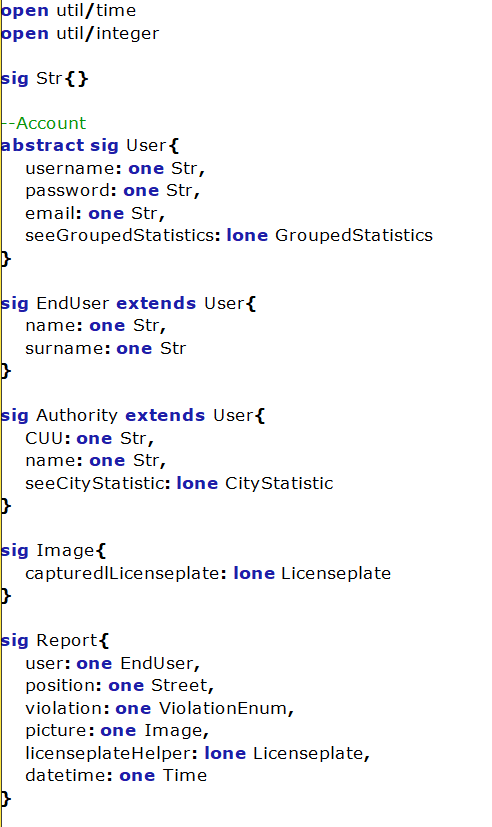
\includegraphics[width=0.9\linewidth, height=0.8 \textheight]{Images/Alloy/codealloy1}
	\caption{Signature 1}
	\label{Signature 1}
\end{figure}

\begin{figure}[h]
	\centering
	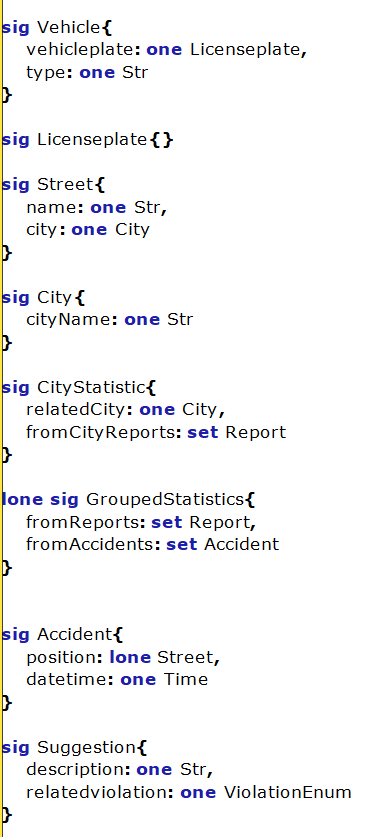
\includegraphics[width=0.5\linewidth, height=0.65\textheight]{Images/Alloy/codealloy2}
	\caption{Signature 2}
	\label{Signature 2}
\end{figure}

\begin{figure}[h]
	\centering
	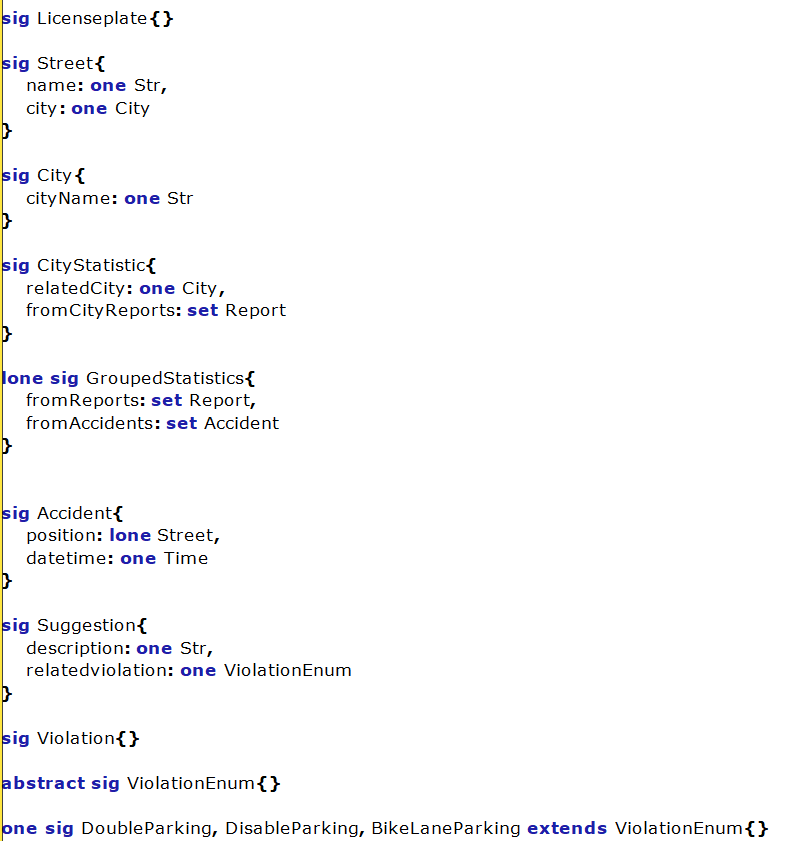
\includegraphics[width=0.9\linewidth, height=0.7\textheight]{Images/Alloy/codealloy3}
	\caption{Signature 3}
	\label{Signature 3}
\end{figure}

\begin{figure}[h]
	\centering
	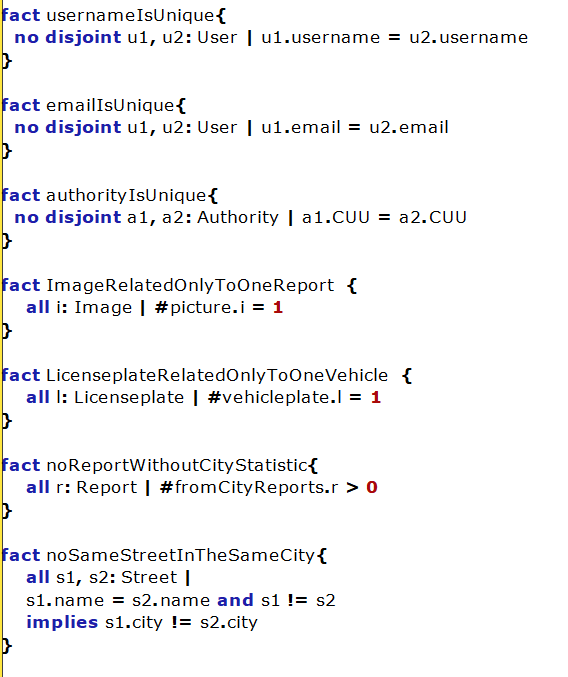
\includegraphics[width=0.9\linewidth, height=0.8\textheight]{Images/Alloy/codealloy4}
	\caption{Pred and Facts 1}
	\label{Pred and Facts 1}
\end{figure}

\begin{figure}[h]
	\centering
	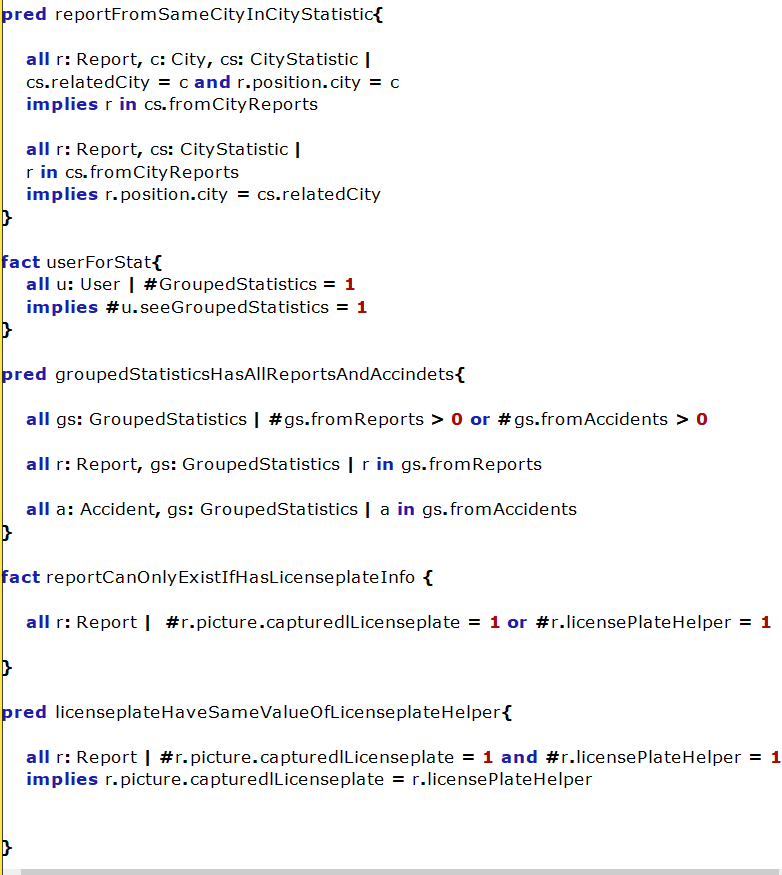
\includegraphics[width=0.9\linewidth, height=0.8\textheight]{Images/Alloy/codealloy5}
	\caption{Pred and Facts 2}
	\label{Pred and Facts 2}
\end{figure}

\begin{figure}[h]
	\centering
	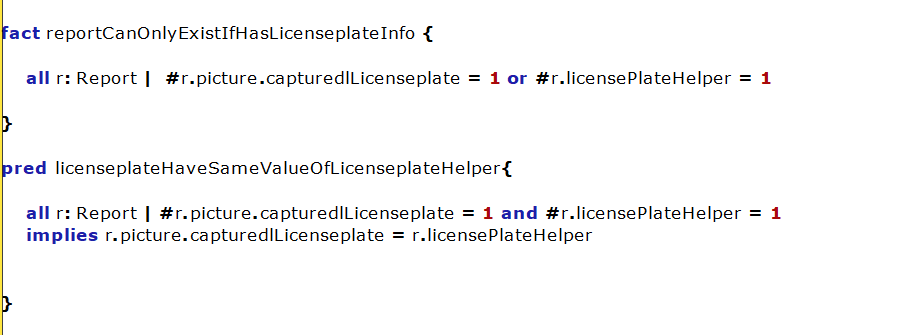
\includegraphics[width=0.9\linewidth, height=0.3\textheight]{Images/Alloy/codealloy6}
	\caption{Pred and Facts 3}
	\label{Pred and Facts 3}
\end{figure}

\begin{figure}[h]
	\centering
	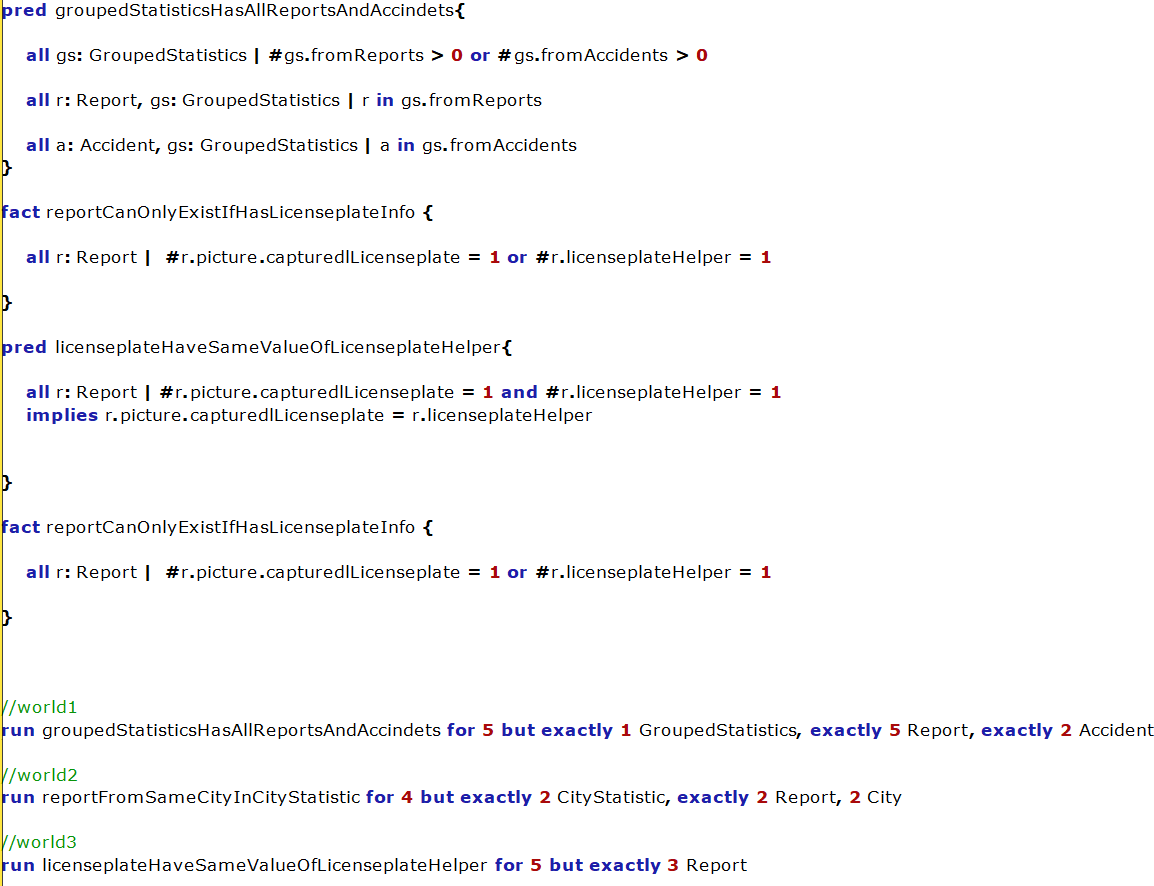
\includegraphics[width=0.95\linewidth, height=0.86\textheight]{Images/Alloy/codealloy7}
	\caption{Pred, Facts and World}
	\label{Pred and Facts and World}
\end{figure}
\FloatBarrier
\subsection{Predicates testing}
\subsubsection{World 1}
Predicate about the aggregation of data coming from reports with the traffic information.

This predicate describes the constraint that the signature that represent statistics can only exist if and only if there is at least one report or accident.
Furthermore all reports and all accidents must be related to statistics.
\begin{figure}[h]
	\centering
	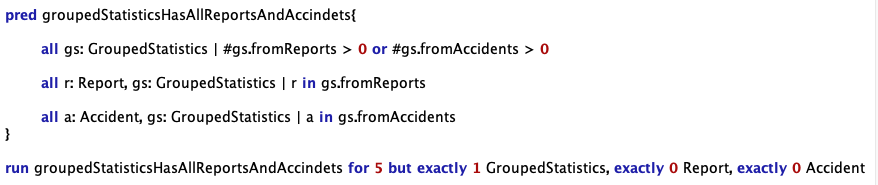
\includegraphics[width=0.9\linewidth, height=0.15\textheight]{Images/Alloy/test-world11}
	\caption{Pred 1}
	\label{Pred 1}
\end{figure}
\FloatBarrier
To show that the predicate works as expected, we have run the predicate with with inconsistent number of sig entities: exactly of  0 reports and 0 accidents but 1 GroupedStatistic
\begin{figure}[h]
	\centering
	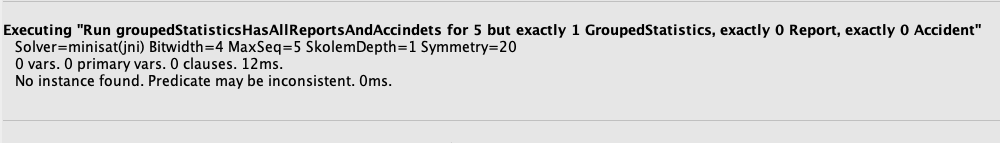
\includegraphics[width=0.9\linewidth, height=0.12\textheight]{Images/Alloy/test-world12}
	\caption{Result pred 1}
	\label{Result pred 1}
\end{figure}
\FloatBarrier
\newpage
The following represented world is generated from the following run: run groupedStatisticsHasAllReportsAndAccindets for 5 but exactly 1 GroupedStatistics, exactly 5 Report, exactly 2 Accident
\begin{figure}[h]
	\centering
	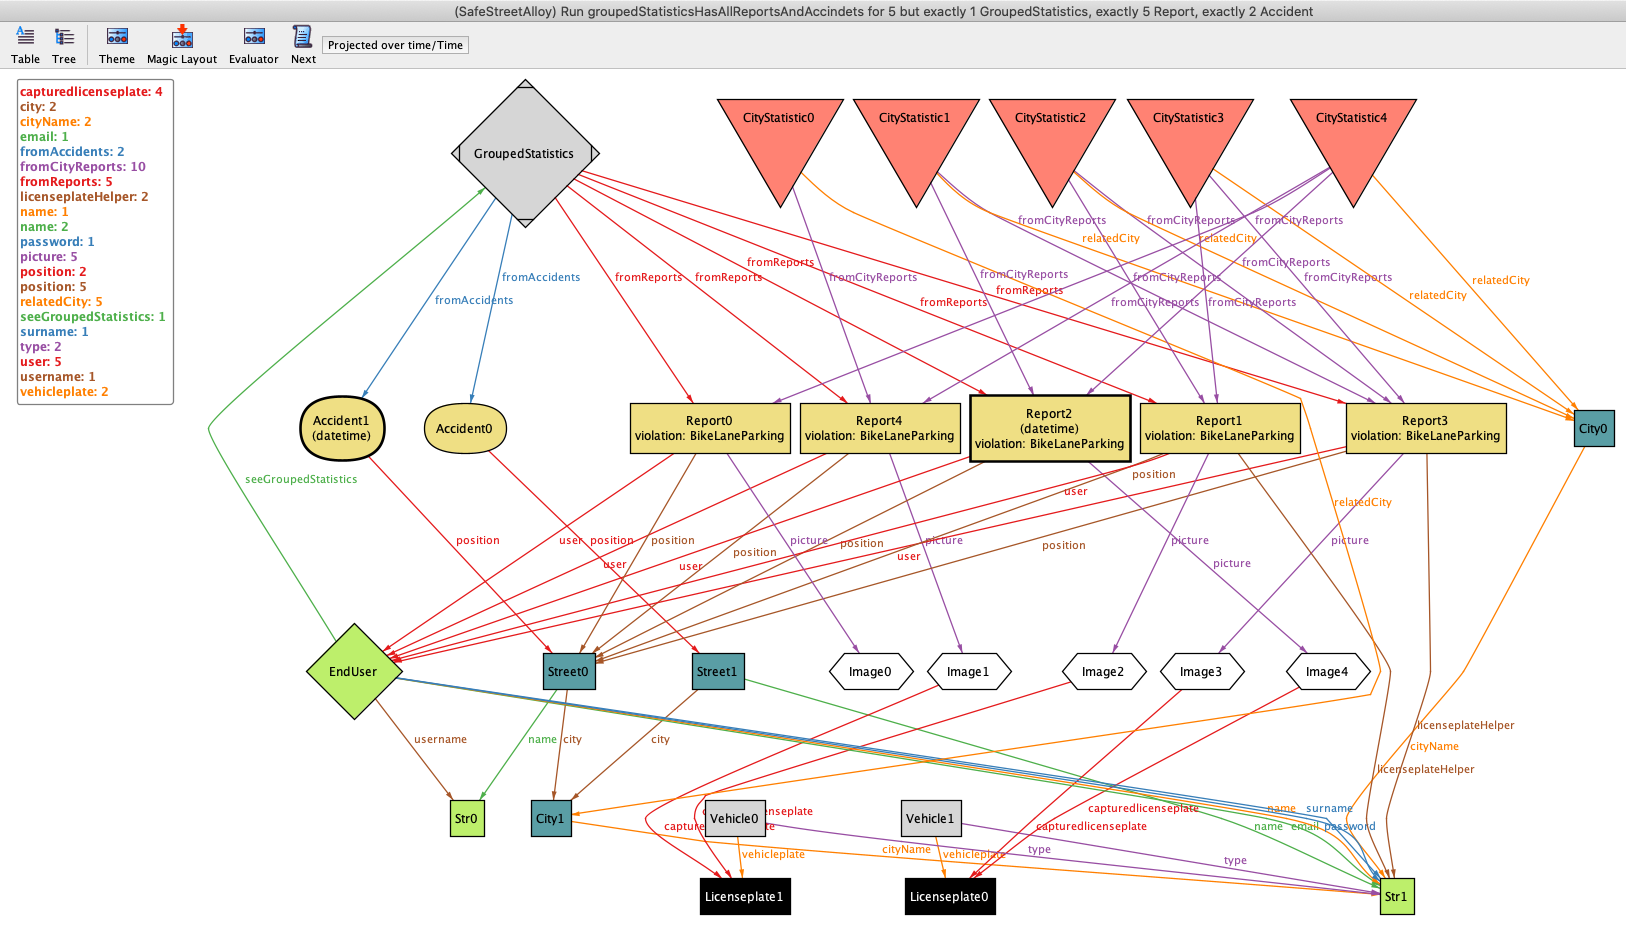
\includegraphics[width=0.9\linewidth, height=0.5\textheight]{Images/Alloy/world1}
	\caption{World 1 generated by pred 1}
	\label{World1 }
\end{figure}
\FloatBarrier
\newpage
\subsubsection{World 2}
Consistency between city and statistics.

This predicate describes the constraint that the signature that represent statistics specific about a city and all reports about all streets of the city must be related.
\begin{figure}[h]
	\centering
	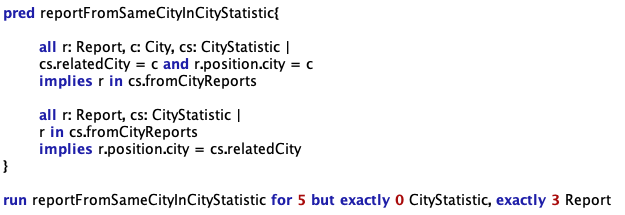
\includegraphics[width=0.9\linewidth, height=0.15\textheight]{Images/Alloy/test-world21}
	\caption{Pred 2}
	\label{Pred 2}
\end{figure}
\FloatBarrier
To show that the predicate works as expected, we have run the predicate with with inconsistent number of sig entities: exactly 0 CityStatistic, exactly 3 Report.
\begin{figure}[h]
	\centering
	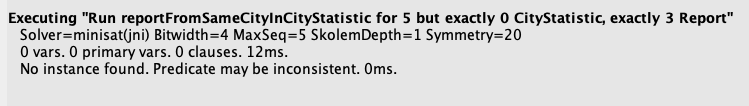
\includegraphics[width=0.9\linewidth, height=0.11\textheight]{Images/Alloy/test-world22}
	\caption{Result pred 2}
	\label{Result pred 2}
\end{figure}
\FloatBarrier
\newpage
The following represented world is generated from the following run: run reportFromSameCityInCityStatistic for 4 but exactly 2 CityStatistic, exactly 2 Report, 2 City
\begin{figure}[h]
	\centering
	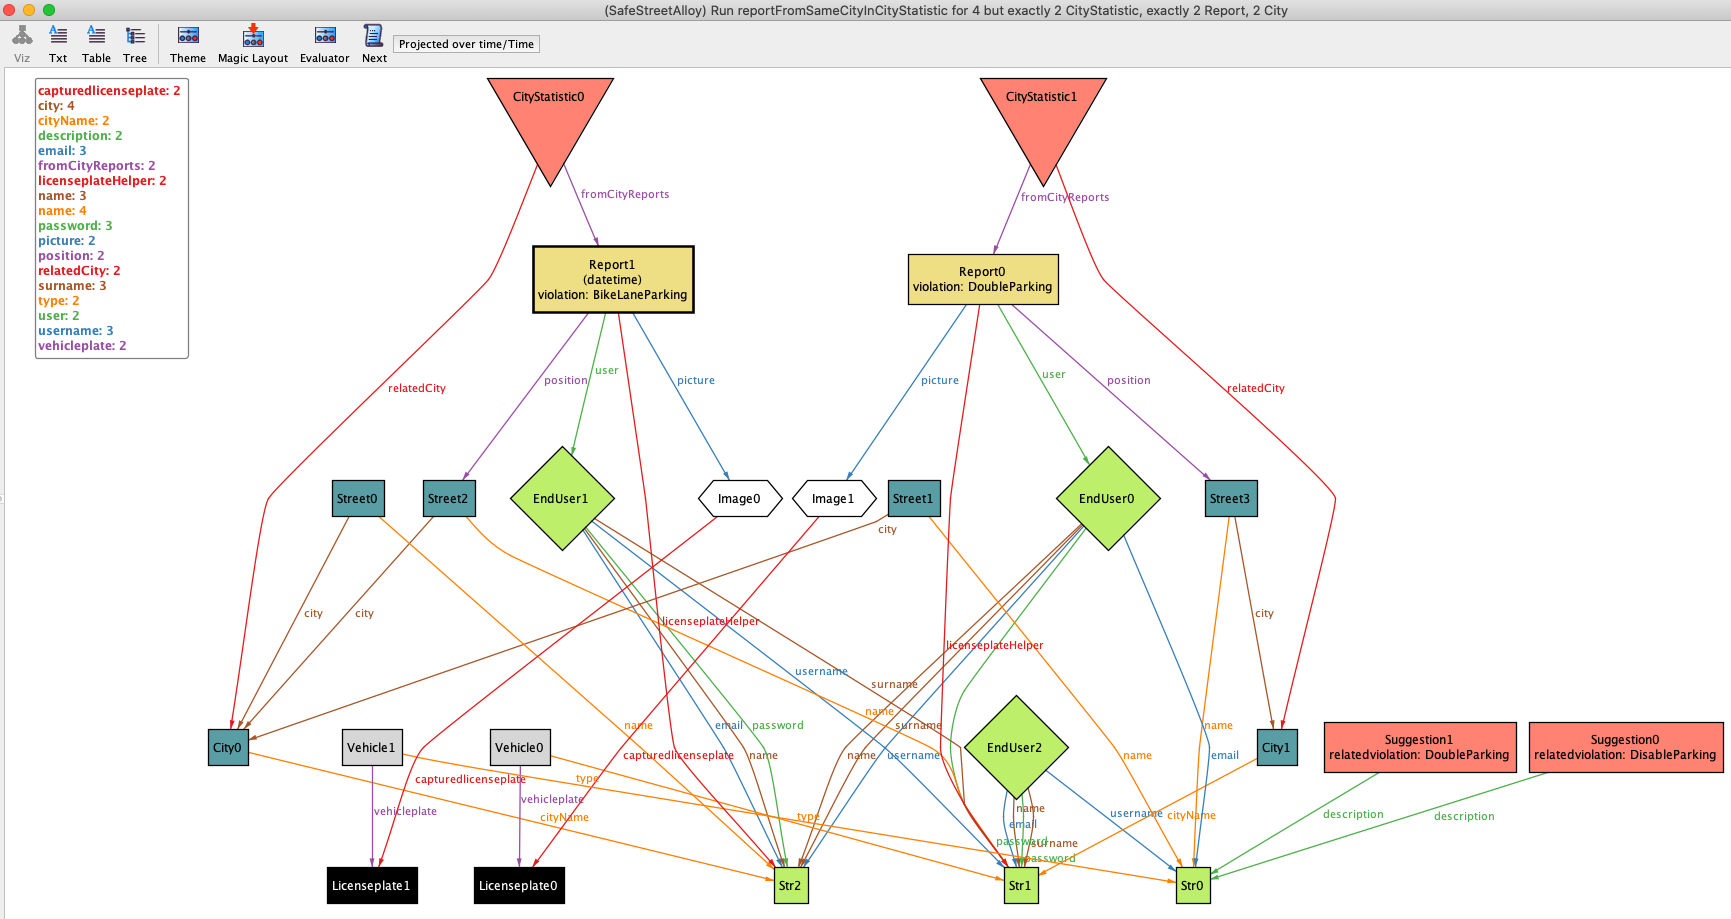
\includegraphics[width=1\linewidth, height=0.47\textheight]{Images/Alloy/world2}
	\caption{World 2}
	\label{World2}
\end{figure}
\FloatBarrier
\newpage
\subsubsection{World 3}
Predicate that test if the licenseplate retrieve from SafeStreets is the same suggested by the user.
\begin{figure}[h]
	\centering
	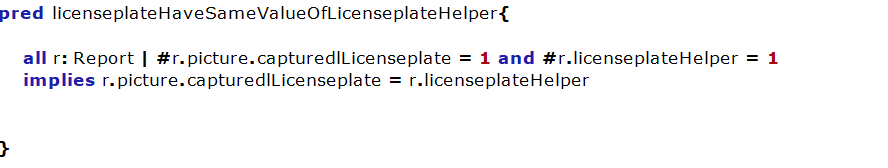
\includegraphics[width=0.9\linewidth, height=0.15\textheight]{Images/Alloy/predworld31}
	\caption{Predicate 3}
	\label{Pred 3}
\end{figure}

\begin{figure}[h]
	\centering
	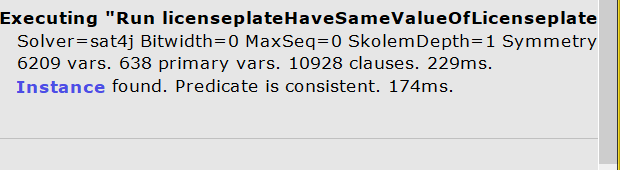
\includegraphics[width=0.8\linewidth, height=0.11\textheight]{Images/Alloy/predworld32}
	\caption{Result pred 3}
	\label{Result pred 3}
\end{figure}
\FloatBarrier
\newpage
The following represented world is generated from the following run: run licenseplateHaveSameValueOfLicenseplateHelper for 5 but exactly 3 Report
\begin{figure}[h]
	\centering
	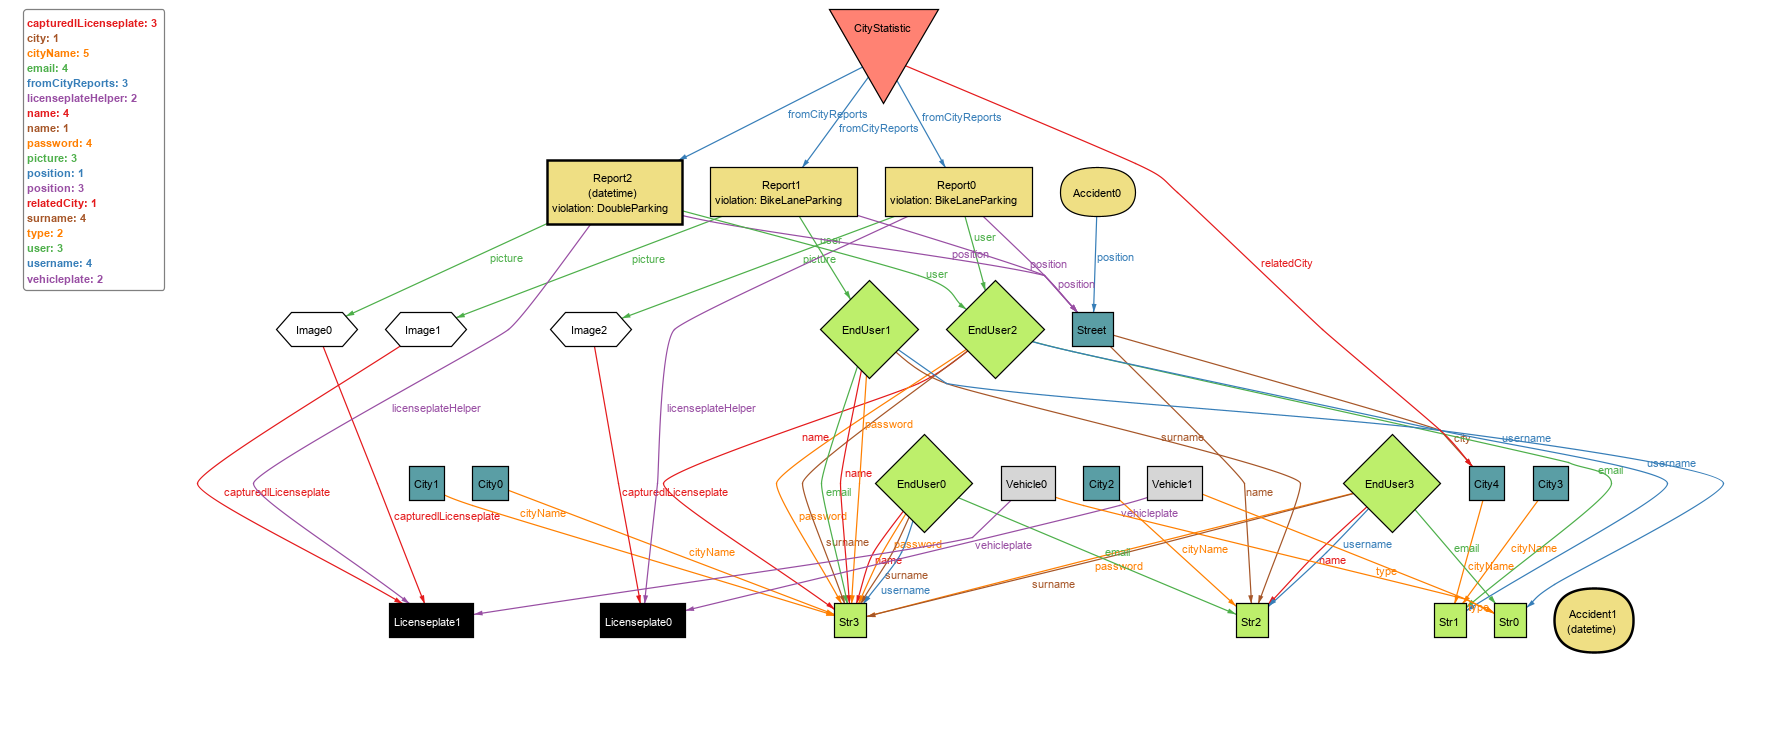
\includegraphics[width=1.1\linewidth, height=0.55\textheight]{Images/Alloy/world3alloy}
	\caption{World 3}
	\label{World3}
\end{figure}


%------------------------------------------------------------------------------------------------------------------------------------------------
\clearpage
{\color{Blue}{\section{Effort Spent}}}
\label{sect:effort}
\hfill
\subsubsection{Ivan Cavadini}
\hfill
\begin{center}
	\begin{tabular}{ | l | p{6cm} | } 
		\hline
		TASK & TIME \\ 
		\hline
		Purpose & 2h  \\ 
		\hline
		Scope & 2h  \\ 
		\hline
		Definitions, Acronyms, Abbreviations & 1h \\ 
		\hline
		Overview & 3h \\ 
		\hline
		Runtime view & 10h \\ 
		\hline
		Requirements traceability & 1h \\ 
		\hline
		Various & 5h  \\ 
		\hline
		TOTAL & 24h \\ 
		\hline
	\end{tabular}
\end{center}
\hfill
\newpage
\subsubsection{Nicolò Molinari}
\hfill
\begin{center}
	\begin{tabular}{ | l | p{6cm} | } 
		\hline
		TASK & TIME \\ 
		\hline
		Component view & 12h  \\ 
		\hline
		Deployment view & 3h  \\ 
		\hline
		Revision history & 0.5h \\ 
		\hline
		Component interfaces & 3h \\ 
		\hline
		Implementation, integration and test & 3h \\ 
		\hline
		Database structure & 1h   \\ 
		\hline
		Various & 4h \\ 
		\hline
		TOTAL & 26.5h \\ 
		\hline
	\end{tabular}
\end{center}
\hfill
\newpage
\subsubsection{Luigi Pederzani}
\hfill
\begin{center}
	\begin{tabular}{ | l | p{6cm} | } 
		\hline
		TASK & TIME \\ 
		\hline
		Revision history & 2h  \\ 
		\hline
		Selected architectural styles and pattern & 8h  \\ 
		\hline
		Other design decisions  & 4h \\ 
		\hline
		User characteristics & 4h \\ 
		\hline
		User Interface design & 5h \\ 
		\hline
		Various & 1.5h  \\ 
		\hline
		TOTAL & 24.5h \\ 
		\hline
	\end{tabular}
\end{center}


\newpage
\subsection{Versions}
\hfill
\hfill
\begin{center}
	\begin{tabular}{ | l | p{6cm} | } 
		\hline
		VERSIONS & DESCRIPTION  \\ 
		\hline
		1.0 & Introduction creation   \\ 
		\hline
		1.1 & Introduction review  \\ 
		\hline
		2.0 & Overview draft \\ 
		\hline
		2.1 & Database structure \\ 
		\hline
		2.2 & Added class diagram \\ 
		\hline
		2.3 & Added component view   \\ 
		\hline
		2.4 & Added runtime view (sequence diagrams)  \\ 
		\hline
		2.5 & Creation of component interfaces \\ 
		\hline
		3.0 & Writing out Selected architectural styles and patterns \\ 
		\hline
		3.1 & Added description of Other design decisions \\ 
		\hline
		4.0 & Creation of UI mocks  \\ 
		\hline
		4.1 & Added screens routing \\ 
		\hline
		5.0 & First draft of Requirements traceability \\ 
		\hline
		5.1 & Requirements traceability correction \\ 
		\hline
		6.0 & Writing out Implementation \\ 
		\hline
		6.1 & Writing out Test \\ 
		\hline
		7.0 & Document review \\ 
		\hline
		7.1 & Final version \\ 
		\hline
	\end{tabular}
\end{center}

\subsection{Used Tools}

\begin{itemize}
	\item TeXstudio 2.12.14
	\item Magic Draw 19.0
	\item MockFlow
	\item Dropbox Paper
\end{itemize}



%------------------------------------------------------------------------------------------------------------------------------------------------
\clearpage
\addcontentsline{toc}{section}{References}
\bibliographystyle{plain}
\bibliography{main}
%------------------------------------------------------------------------------------------------------------------------------------------------




\end{document}
